\documentclass[twocolumn, 11pt]{scrartcl}
\usepackage[narrow-margins]{jamiepack}
\addbibresource{bib.bib}

% This is for the PDF metadata
\title{Isogeny Pullbacks of Elliptic Codes}
\author{Jamie Low Jiaqi}

% Uncomment to check spacing
\raggedbottom

\begin{document}

% This is for \maketitle
\title{\textbf{Isogeny Pullbacks of Elliptic Codes: Quasi-Cyclic, Iso-Dual and MDS Codes with Matrix-Product Structure}}
\author{\textbf{Jamie Low Jiaqi}\\School of Physical and Mathematical Sciences, Nanyang Technological University, Singapore}
\date{November 2026}
\maketitle

% This is for the page headers
\title{Isogeny Pullbacks of Elliptic Codes}
\author{Jamie Low Jiaqi}
\date{}

\usection{Abstract}

Isogenies of elliptic curves are central to post-quantum cryptography, but have so far played almost no role in coding theory. We pull back an elliptic code $C=C_\mcL(D,G)$ along a separable isogeny $\varphi:\mcE_1\to\mcE_2$ with cyclic kernel of order $\ell$, obtaining the \textit{pullback code} $\varphi^*C=C_\mcL(\varphi^*D,\varphi^*G)$ of length $\ell n$. We show that $\varphi^*C$ is quasi-cyclic of co-index $\ell$ with the same rate and relative designed distance as $C$, and that it inherits iso-duality. When $\ell\mid q-1$, $\varphi^*C$ is monomially equivalent to a matrix-product code whose constituents are scalings of $\ell$ twisted elliptic codes on $\mcE_2$, which yields a subset-sum condition that every MDS pullback code satisfies. Combining pullbacks with index-two subgroups, we construct quasi-cyclic MDS elliptic codes. From the hulls of pullback codes, we also obtain quasi-cyclic entanglement-assisted quantum codes with prescribed entanglement.

\textbf{Keywords:} elliptic curves, isogenies, algebraic geometry codes, quasi-cyclic codes, matrix-product codes, MDS codes, hulls, entanglement-assisted quantum codes

\section{Introduction} \label{section:introduction}

Algebraic geometry (AG) codes were introduced by Goppa \cite{goppa1983algebraico} in the early 1980s. Their codewords are evaluations of functions in a Riemann--Roch space at rational points of a curve. They generalise the generalised Reed--Solomon (GRS) codes \cite{macwilliams1977theory} and have Singleton defect at most the genus of the curve \cite{stichtenoth2009algebraic}. They garnered strong interest after some families of AG codes were shown to beat the Gilbert--Varshamov bound \cite{tsfasman1982modular}.

Elliptic curves give the simplest AG codes inequivalent to GRS codes. They are the only algebraic curves whose points canonically form an abelian group, so conditions on the defining divisors become conditions on sums of points under the group law. This reduces the MDS property to a subset-sum problem \cite{munuera1993mds,li2015minimum}, and has led to MDS \cite{wang2025nonrs}, iso-dual \cite{zhu2026isodual} and self-dual \cite{jin2019selfdual} elliptic codes, with applications to quantum codes \cite{sok2021new,zhu2026isodual}.

Quasi-cyclic (QC) codes \cite{ling2001algebraic} arise on AG codes from curve automorphisms. Tong and Ding \cite{tong2013quasicyclic} built QC elliptic codes from automorphisms fixing the point at infinity, which have order at most 6. Translations \cite{ma2023automorphism} have larger orders, but they move the point at infinity, so the usual one- and two-point divisors are not invariant.

Isogenies are morphisms of elliptic curves respecting the group law, and are a source of divisors invariant under translations.  They are central to post-quantum cryptography \cite{NISTPQC-ADD-R3:SQIsign26,basso2026prism}, yet virtually unseen in coding theory. Given a separable isogeny $\varphi:\mcE_1\to\mcE_2$ with cyclic kernel $K$ of order $\ell$ and an elliptic code $C=C_\mcL(D,G)$ on $\mcE_2$, we study the \textbf{pullback code} $\varphi^*C:=C_\mcL(\varphi^*D,\varphi^*G)$. Translations by $K$ preserve $\varphi^*D$ and $\varphi^*G$, and hence act on $\varphi^*C$. We show the following.
\begin{itemize}
    \item $\varphi^*C$ is an $[\ell n,\ell k,\geq\ell(n-k)]_q$ QC code of co-index $\ell$ (\Cref{theorem:pullback}), whose $K$-fixed subcode is the $\ell$-fold repetition of $C$ (\Cref{proposition:pullback-fixed}), and which inherits iso-duality from $C$ (\Cref{corollary:pullback-isodual}).
    \item If $\ell\mid q-1$, then $\varphi^*C$ is monomially equivalent to a matrix-product code whose constituents are scalings of twists $C_\mcL(D,G_j)$ of $C$ (\Cref{theorem:pullback-split}). If $\varphi^*C$ is MDS, so is every twist (\Cref{corollary:pullback-twists-mds}).
    \item Modifying the index-two method of \cite{wang2025nonrs}, pullbacks give QC MDS elliptic codes (\Cref{construction:index-two-pullback}, \Cref{example:mds-qc}).
    \item The hull of $\varphi^*C$ splits along its twists, and scaling whole fibres gives QC EAQECCs with prescribed entanglement (\Cref{theorem:hull-decomposition,theorem:qc-hv}, \Cref{corollary:qc-eaqecc}).
\end{itemize}

\Cref{section:preliminaries} gives background, \Cref{section:group-law} collects tools from the group law, and \Cref{section:isogenies,section:hulls} contain our results.

\section{Preliminaries} \label{section:preliminaries}

We summarise key definitions and results pertaining to divisors on algebraic curves, elliptic curves and their isogenies, and AG codes. For a more detailed description with proofs of results, we refer the reader to the following comprehensive standard references, which our exposition is based on:
\begin{itemize}
    \item Silverman's book \cite{silverman2009arithmetic} for basic arithmetic geometry, with a focus on elliptic curves;
    \item Stichtenoth's book \cite{stichtenoth2009algebraic} for algebraic function fields and algebraic geometry (AG) codes.
\end{itemize}
Henceforth, let $q=p^m$ denote a prime power.

\subsection{Divisors} \label{section:divisors}

Let $\mcC$ be a smooth projective, geometrically irreducible curve of genus $g$ over $\bbF_q$, which we identify with its set of $\Fbar{q}$-points. A point of $\mcC$ is \textbf{$\bbF_q$-rational} if its coordinates lie in $\bbF_q$, and the set of $\bbF_q$-rational points is denoted by $\mcC(\bbF_q)$.

A \textbf{divisor} of $\mcC$ is an element $D$ of the free abelian group $\Div\mcC=\bbZ[\mcC]$ over the points of $\mcC$. In other words, it is a formal sum
\[ D=\sum_{P\in\mcC} n_P\cdot(P),\quad n_P\in\bbZ \]
where all but finitely many $n_P$ are zero. Its \textbf{support} and \textbf{degree} are, respectively,
\[ \supp D=\set{P\in\mcC:n_P\neq0} \qand \deg D=\sum_{P\in\mcC} n_P. \]
A partial ordering on $\Div\mcC$ is defined by
\[ \sum_{P\in\mcC} n_P(P)\leq\sum_{P\in\mcC} n'_P(P) \qiff \forall P\in\mcC:\quad n_P\leq n'_P. \]
$D$ is called \textbf{effective} if $D\geq 0$.

The \textbf{function field} $\bbF_q(\mcC)$ of $\mcC$ is the field of rational functions on $\mcC$ defined over $\bbF_q$. For $f\in\bbF_q(\mcC)^*$, set
\[ \div f:=\sum_{P\in\mcC} \ord_P(f)\cdot(P),\quad\text{where} \]
\begin{itemize}
    \item $\ord_P(f)=n\in\bbZ^+$ if $f$ has a zero of order $n$ at $P$;
    \item $\ord_P(f)=-n\in\bbZ^-$ if $f$ has a pole of order $n$ at $P$;
    \item $\ord_P(f)=0$ otherwise.
\end{itemize}
Such divisors are called \textbf{principal} and form a subgroup $\PDiv\mcC$ of the degree-0 divisors $\Div^0\mcC$. Two divisors (of any degree) are called \textbf{equivalent}, written $A\sim B$, if they differ by a principal divisor. The \textbf{Jacobian} of $\mcC$ is the quotient $\Jac\mcC:=\Div^0\mcC/\PDiv\mcC$.\footnote{More precisely, this quotient is called the Picard group of degree 0, but this is isomorphic to the Jacobian variety.}

Given a divisor $G\in\Div\mcC$, we construct the \textbf{Riemann--Roch space}
\[ \mcL(G):=\set{f\in\bbF_q(\mcC)^*:\div f\geq-G}\cup\set0. \]
This is a finite-dimensional vector subspace of $\bbF_q(\mcC)$, and we denote its dimension by $\ell(G)$. The Riemann--Roch Theorem \cite[\S1.5]{stichtenoth2009algebraic} gives us $\ell(G)\geq\deg G+1-g$, with equality when $\deg G>2g-2$.

The \textbf{space of differential forms} $\Omega_\mcC$ on $\mcC$ is the $\bbF_q$-vector space generated by symbols of the form $\df$ for $f\in\bbF_q(\mcC)$, subject to the relations
\[ \dx[(f+g)]=\df+\dg,\quad \dx[(fg)]=f\,\dg+g\,\df,\quad \da=0 \]
for all $f,g\in\bbF_q(\mcC)$ and $a\in\bbF_q$. Around a point $P\in\mcC$, every $\omega\in\Omega_\mcC^*$ can be written uniquely as
\[ \omega=\sum_{n=m}^\infty a_nt^n\dt\quad\text{for some  } \begin{cases}
        t\in\bbF_q(\mcC),\ \ord_P(t)=1, \\
        a_n\in\bbF_q,\ a_m\neq 0,\ m\in\bbZ.
    \end{cases} \]
For $\omega\in\Omega_\mcC^*$, set $\ord_P(\omega):=m$, $\Res_P(\omega):=a_{-1}$ (or 0 if $m\geq 0$),
\vspace{-6pt}
\begin{align*}
    \div\omega&:=\sum_{P\in\mcC}\;\ord_P(\omega)\cdot(P),\quad\text{and}\\
    \Omega(G)&:=\set{\omega\in\Omega_\mcC^*:\div\omega\geq G}\cup\set0.
\end{align*}
Such divisors $\div\omega$ are called \textbf{canonical}. They all lie in one equivalence class and have degree $2g-2$ \cite[\S1.5]{stichtenoth2009algebraic}.

Finally, let $\varphi:\mcC_1\to\mcC_2$ be a nonconstant morphism of curves, defined over $\bbF_q$. It induces a \textbf{pullback} map $\varphi^*$ on functions, differentials, and divisors, defined by
\begin{alignat*}{2}
    \bbF_q(\mcC_2)&\to\bbF_q(\mcC_1), & \quad f &\mapsto f\circ\varphi \\
    \Omega_{\mcC_2}&\to\Omega_{\mcC_1}, & \quad \df &\mapsto \dx[(f\circ\varphi)] \\
    \Div\mcC_2&\to\Div\mcC_1, & \quad \sum_{Q\in\mcC_2} n_Q(Q) &\mapsto \sum_{Q\in\mcC_2} n_Q \sum_{\mathclap{P\in\varphi^{-1}(Q)}} e_P(P)
\end{alignat*}
where $e_P$ denotes the ramification index of $P\in\mcC_1$ in $\varphi^{-1}(Q)$, the \textbf{fibre} over $Q\in\mcC_2$. On functions, $\varphi^*$ is an injective field homomorphism, so $\varphi$ induces a finite field extension $\varphi^*\bbF_q(\mcC_2)\leq\bbF_q(\mcC_1)$, whose degree is the \textbf{degree} $\deg\varphi$ of the morphism. We call $\varphi$ \textbf{separable} if this extension is separable.

Some key properties of $\varphi^*$, which we use freely in our proofs, are as follows.
\begin{itemize}
    \item On divisors, $\varphi^*$ preserves the partial order and multiplies degrees by $\deg\varphi$.
    \item $\varphi^*$ is compatible with principal divisors, in the sense that $\varphi^*\div f=\div\varphi^*f$.
    \item $\varphi^*$ sends equivalent divisors to equivalent divisors.
    \item $\varphi^*$ induces a homomorphism $\Jac\mcC_2\to\Jac\mcC_1$.
    \item $\varphi^*$ maps $\mcL(G)$ into $\mcL(\varphi^*G)$ for every $G\in\Div\mcC_2$.
    \item If $\varphi$ is an automorphism of $\mcC$, then $\varphi^*(P)=\pa[\big]{\varphi^{-1}(P)}$, so $\varphi^*$ merely permutes the points of a divisor and preserves effectiveness.
\end{itemize}

\subsection{Elliptic curves} \label{section:elliptic-curves}

An \textbf{elliptic curve} $\mcE$ over $\bbF_q$ is a smooth projective curve of genus 1 with an $\bbF_q$-rational point. Equivalently, $\mcE$ is the set of points $(x,y)\in\Fbar{q}^2$ satisfying an equation of the form
\[ y^2+a_1xy+a_3y=x^3+a_2x^2+a_4x+a_6, \quad a_i\in\bbF_q \eqlabel{eqn:ec} \]
together with a point at infinity $\infty$, provided that no point is singular. Denote $\mcE(\bbF_q):=(\mcE\cap\bbF_q^2)\cup\set\infty$ and $\mcE(\bbF_q)^*:=\mcE\cap\bbF_q^2$ for the set of all (resp. affine) $\bbF_q$-rational points. The cardinality $N:=\#\mcE(\bbF_q)$ is constrained by the Hasse--Weil bound \cite[\S~V.1]{silverman2009arithmetic}
\[ \abs{N-(q+1)}\leq\floor{2\sqrt q}. \]
The points of $\mcE$ form an abelian group $(\mcE,\oplus)$ with identity $\infty$, where the group addition $\oplus$ is governed by the equations in \cite[\S~III.2]{silverman2009arithmetic} and visualised in \Cref{fig:elliptic-group-law}. As is standard in the literature, $[m]P$ denotes the $m$-fold sum $P\oplus\cdots\oplus P$ for $m\in\bbN$, and $[-m]P:=\ominus[m]P$.

\begin{figure}
    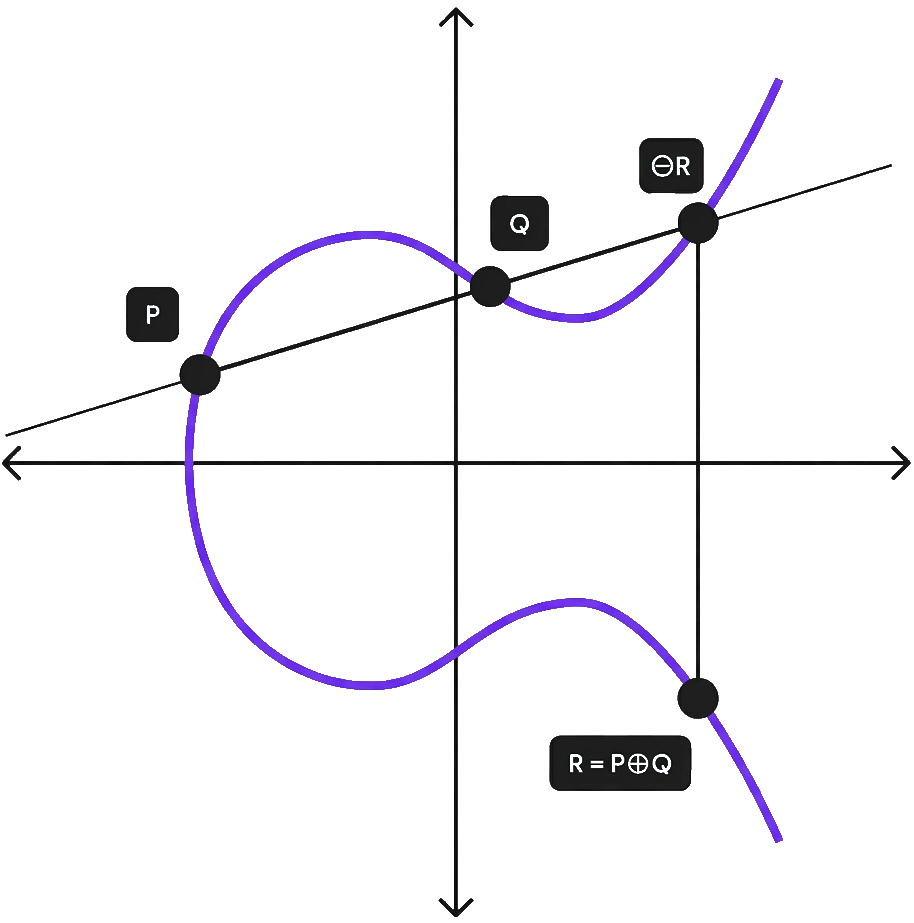
\includegraphics[width=0.3\textwidth]{assets/elliptic-group-law}
    \figcaption{The group law of an elliptic curve $\mcE$ over $\bbR$ \cite{elusiv_ecc_2023}}
    \label[figure]{fig:elliptic-group-law}
\end{figure}

We now specialise \Cref{section:divisors} to $\mcC=\mcE$, where $g=1$. The function field $\bbF_q(\mcE)$ is the field $\bbF_q(x,y)$, where $x$ is transcendental over $\bbF_q$ and $y$ is algebraic over $\bbF_q(x)$ subject to \Cref{eqn:ec}. The Riemann--Roch Theorem gives us $\ell(G)\geq\deg G$, with equality when $\deg G\geq1$. The sets of canonical and principal divisors coincide \cite[Cor.~1.4.12]{stichtenoth2009algebraic}. Moreover, the Jacobian $\Jac\mcE$ is famously isomorphic to $\mcE$ (cf. \Cref{section:group-law}).

The \textbf{sum map} $\Sigma$ on divisors evaluates the formal sum using the elliptic group law and is denoted by
\[ \Sigma(D):=\bigoplus_{P\in\mcE} [n_P]P. \]

\subsection{Isogenies} \label{section:isogeny-background}

Let $\mcE_1$ and $\mcE_2$ be elliptic curves over $\bbF_q$. An \textbf{isogeny} $\varphi:\mcE_1\to\mcE_2$ is a nonconstant morphism of curves that fixes $\infty$. Such a map is automatically a surjective group homomorphism with finite kernel. We assume henceforth that every isogeny is \textbf{separable}, so that $\ell=\#\ker\varphi$ and $e_P=1$ for all $P$. 

Every finite subgroup $K\leq\mcE_1$ that is stable under the Frobenius map is the kernel of a separable isogeny $\mcE_1\to\mcE_1/K$ defined over $\bbF_q$, which can be computed explicitly using V\'elu's formulae \cite{velu1971isogenies}. In particular, every subgroup $K\leq\mcE_1(\bbF_q)$ arises in this way.

Every isogeny $\varphi$ admits a \textbf{dual isogeny} $\hat\varphi:\mcE_2\to\mcE_1$, which satisfies $\hat\varphi\circ\varphi=[\ell]$ and $\varphi\circ\hat\varphi=[\ell]$. Its construction implies that $\Sigma(\varphi^*B)=\hat\varphi(\Sigma(B))$ for every $B\in\Div^0\mcE_2$.

For more details on isogenies and proofs of the above claims, see \cite[\S~III.4--6]{silverman2009arithmetic}.

\subsection{Algebraic geometry codes} \label{section:ecc}

Let $n\in\bbZ^+$ and $D,G\in\Div\mcC$ be two divisors such that $\supp D\cap\supp G=\emptyset$ and $D=(P_1)+\cdots+(P_n)$ is a sum of $n$ distinct $\bbF_q$-rational points. Fixing an ordering of $\supp D$, we adopt the notation
\[ f(D):=(f(P_1),\hdots,f(P_n))\in\bbF_q^n\qtx{for}f\in\mcL(G). \]
The \textbf{AG code} associated with $D$ and $G$ is
\[ C_\mcL(D,G):=\set{f(D):f\in\mcL(G)}. \]
If $\deg G<n$, then evaluation at $D$ is injective on $\mcL(G)$, and $C_\mcL(D,G)$ is an $[n,k,d]_q$ code with $k=\ell(G)\geq\deg G+1-g$ and $d\geq n-\deg G$ \cite[Thm.~2.2.2]{stichtenoth2009algebraic}. The quantity $d^*:=n-\deg G$ is called the \textbf{designed distance}.

The Euclidean dual code $C_\mcL(D,G)^{\perp_\rmE}$ of $C_\mcL(D,G)$ is
\[ C_\Omega(D,G)=\set*{(\Res_{P_1}(\omega),\hdots,\Res_{P_n}(\omega)):\omega\in\Omega(G-D)}, \]
as proven in \cite[Prop.~8]{o2008key}. Choose $t\in\bbF_q(\mcC)$ such that $\ord_{P_i}(t)=1$ for $1\leq i\leq n$. Then, the differential $\eta:=\dt/t$ has the property that every $\omega\in\Omega(G-D)$ can be written as $f\eta$ for some $f\in\mcL(H)$, where $H=D-G+\div\eta$ \cite[\S8.1]{stichtenoth2009algebraic}. As such, we have the beautiful result that $C_\Omega(D,G)=C_\mcL(D,H)$, so the dual of an AG code is again an AG code.

An \textbf{elliptic code} is an AG code on an elliptic curve $\mcE$ with $1\leq\deg G\leq n-1$. By the above, it is an $[n,k,d]_q$ code with $k=\deg G$ and $d\geq n-k$, so its Singleton defect is at most 1. Its dual $C_\mcL(D,H)$ is also an elliptic code, as $\deg H=n-k$. A code is called \textbf{one-point} (resp. \textbf{two-point}) if $\supp G$ contains exactly one (resp. two) points.

We now recall some terminology for codes.
\begin{itemize}
    \item For $\bfv\in(\bbF_q^*)^n$ and a code $C\subseteq\bbF_q^n$, write $\bfv\star C:=\set{(v_1c_1,\hdots,v_nc_n):\bfc\in C}$ for the \textbf{scaling} of $C$ by $\bfv$.
    \item Two codes are \textbf{monomially equivalent} if one is obtained from the other by a scaling and a coordinate permutation.
    \item An $[n,k,d]_q$ code is \textbf{maximum distance separable} (MDS) if $d=n-k+1$. It is \textbf{near-MDS} if $d=n-k$ and its dual also has Singleton defect 1 \cite{dodunekov1995near}. Hence, every elliptic code is either MDS or near-MDS.
    \item A code $C$ is \textbf{self-dual} if $C^{\perp_\rmE}=C$, and \textbf{iso-dual} if $C^{\perp_\rmE}=\bfv\star C$ for some $\bfv\in(\bbF_q^*)^n$ \cite{jin2019selfdual,zhu2026isodual}. In both cases, we necessarily have $n=2k$.
    \item A code of length $mt$ is \textbf{quasi-cyclic} (QC) of index $m$ and co-index $t$ if it is invariant under a coordinate permutation consisting of $m$ disjoint $t$-cycles \cite{ling2001algebraic,tong2013quasicyclic}. Equivalently, after reordering coordinates, it is invariant under $m$-fold cyclic shifts.
    \item Given codes $C_0,\hdots,C_{s-1}\subseteq\bbF_q^n$ and a matrix $\bfA\in\bbF_q^{s\times t}$, the \textbf{matrix-product code} \cite{blackmore2001matrix} is the code of length $nt$
    \[ (C_0,\hdots,C_{s-1})\cdot\bfA:=\set*{(\bfc_0,\hdots,\bfc_{s-1})\bfA:\bfc_j\in C_j}, \]
    where the $\bfc_j$ are column vectors, concatenated to form an $n\times s$ matrix.
\end{itemize}

\subsection{Hulls and entanglement-assisted quantum codes} \label{section:hulls-background}

Throughout, $\perp$ denotes the Euclidean dual. The \textbf{hull} of a code $C$ is $\Hull(C):=C\cap C^\perp$. The extreme cases $\Hull(C)=C$ and $\Hull(C)=\set{\bf0}$ are the \textbf{self-orthogonal} and \textbf{linear complementary dual} (LCD) codes respectively. The hull is not invariant under scaling, so equivalent codes may have hulls of different dimensions.

An \textbf{entanglement-assisted quantum error-correcting code} (EAQECC) with parameters $\llbracket n,\kappa,d;c\rrbracket_q$ encodes $\kappa$ logical qudits into $n$ physical qudits with the help of $c$ pre-shared maximally entangled pairs, and has minimum distance $d$ \cite{brun2006correcting}. When $c=0$, it is a quantum stabiliser code. The Singleton bound for EAQECCs reads
\[ 2d\leq n-\kappa+c+2 \qtx{whenever} d\leq\tfrac{n}{2}+1, \]
and an EAQECC achieving it is called \textbf{MDS} \cite{lai2018linear}. EAQECCs can be built from any classical linear code, with the entanglement determined by the hull.

\begin{lemma}{Hull bound \cite[Lem.~16]{chen2023hulls}}{hull-eaqecc}
    Let $C$ be an $[n,k,d]_q$ code and put $h=\dim\Hull(C)$. Then, there exists an EAQECC with parameters $\llbracket n,\;k-h,\;d;\;n-k-h\rrbracket_q$.

    If $C$ is MDS and $d\leq\frac{n}{2}+1$ (equivalently, $k\geq\frac n2$), this EAQECC is also MDS.
\end{lemma}

\section{Exploiting the group law} \label{section:group-law}

The group law on an elliptic curve allows conditions on divisors to be rewritten as conditions on sums of points. This section collects the consequences of this principle that we will use as tools in \Cref{section:isogenies}. They are known, and we state them in the form we need.

Every curve $\mcC$ of genus $g$ carries an abelian variety of dimension $g$, its Jacobian $\Jac\mcC$. What distinguishes genus 1 is that the group structure can be transported from the Jacobian to the curve. Specifically, for an elliptic curve, the \textbf{Abel--Jacobi map}
\[ \mcE\lra\Jac\mcE, \qquad P\longmapsto\br{(P)-(\infty)} \]
is a bijection whose inverse is the sum map $\Sigma$ of \Cref{section:elliptic-curves}, and the group law it induces on $\mcE$ agrees with the geometric one in \cite[\S~III.3]{silverman2009arithmetic}. For $g\geq2$ the group lives on a higher-dimensional variety, and no such translation is available.

\begin{lemma}{Abel--Jacobi \cite[Cor.~III.3.5]{silverman2009arithmetic}}{abel-jacobi}
    $A\in\Div^0\mcE$ is principal if and only if $\Sigma(A)=\infty$.
\end{lemma}

Henceforth we assume, as is standard, that $\supp G\subset\mcE(\bbF_q)$, so that $\Sigma(G)\in\mcE(\bbF_q)$. The first tool decides whether an elliptic code is MDS or near-MDS. We use it to analyse MDS pullback codes in \Cref{corollary:pullback-twists-mds} and \Cref{construction:index-two-pullback}.

\begin{theorem}{Subset-sum criterion \cite{munuera1993mds,li2015minimum}}{mds-criterion}
    Let $C_\mcL(D,G)$ be an elliptic code, with $D=(P_1)+\cdots+(P_n)$ and $k=\deg G$. Then $d=n-k$ if and only if there are $k$ distinct points $P_{i_1},\hdots,P_{i_k}\in\supp D$ with
    \[ P_{i_1}\oplus\cdots\oplus P_{i_k}=\Sigma(G). \eqlabel{eqn:mds-criterion} \]
    Otherwise, $d=n-k+1$, and the code is MDS.
\end{theorem}

Indeed, if \Cref{eqn:mds-criterion} holds, then \Cref{lemma:abel-jacobi} gives a function $f\in\mcL(G)$ with $\div f=\sum_j(P_{i_j})-G$, and $f(D)$ is a codeword of weight $n-k$.

The second tool lets us replace $G$ by any divisor with the same degree and sum. We use it to identify the twists in \Cref{theorem:pullback-split} and to choose convenient divisors in \Cref{example:mds-qc}.

\begin{lemma}{Equivalent divisors \cite[\S~2.2]{stichtenoth2009algebraic}}{equiv-codes} % \cite[Prop.~2.2.14]{stichtenoth2009algebraic}
    If $G$ and $H$ are equivalent divisors whose supports are disjoint from $D$, then $C_\mcL(D,G)$ and $C_\mcL(D,H)$ differ at most by coordinate scaling.
\end{lemma}

\begin{corollary}{Two-point normal form \cite{wang2025nonrs,zhu2026isodual}}{normal-form}
    Let $C_\mcL(D,G)$ be an elliptic code with $k=\deg G$. Let $Q_0,Q_1\in\mcE(\bbF_q)\bs\supp D$ be such that $G':=(k-1)(Q_0)+(Q_1)$ satisfies $\Sigma(G')=\Sigma(G)$. Then $C_\mcL(D,G)$ and $C_\mcL(D,G')$ differ at most by coordinate scaling.
\end{corollary}

\begin{proof}
    $G-G'$ has degree 0 and sum $\infty$, so it is principal by \Cref{lemma:abel-jacobi}. Apply \Cref{lemma:equiv-codes}.
\end{proof}

The third tool is a sufficient condition for iso-duality, which underlies the iso-dual MDS codes of \cite{zhu2026isodual}. We use it in \Cref{corollary:pullback-isodual}.

\begin{lemma}{Iso-dual criterion \cite{zhu2026isodual}}{isodual-criterion}
    Let $C=C_\mcL(D,G)$ be an elliptic code. If $D-2G$ is principal, or equivalently, if $\deg D=2\deg G$ and $\Sigma(D)=[2]\Sigma(G)$, then $C$ is iso-dual.
\end{lemma}

\begin{proof}
    The two conditions are equivalent by \Cref{lemma:abel-jacobi}. By \Cref{section:ecc}, $C^{\perp_\rmE}=C_\mcL(D,H)$ with $H=D-G+\div\eta$. As $\div\eta$ is principal (\Cref{section:elliptic-curves}), $H-G=D-2G+\div\eta$ is principal, so $C_\mcL(D,H)$ is a scaling of $C$ by \Cref{lemma:equiv-codes}.
\end{proof}

The fourth tool concerns automorphisms. For $R\in\mcE(\bbF_q)$, the \textbf{translation} map $\tau_R:P\mapsto P\oplus R$ is an automorphism of $\mcE$ as a curve. $\tau_R^*$ acts by
\[ \bbF_q(\mcE)\ni f\mapsto f\circ\tau_R \qand \Div\mcE\ni(P)\mapsto(P\ominus R),\]
so that
\[ \tau_R^*\mcL(G)=\mcL(\tau_R^*G)\ \ \text{and}\ \ \Sigma(\tau_R^*G)=\Sigma(G)\ominus[\deg G]R.\]

\begin{theorem}{Translation automorphisms \cite{ma2023automorphism}}{translations}
    Let $C:=C_\mcL(D,G)$ be an elliptic code with $k=\deg G$. Suppose $R\in\mcE(\bbF_q)$ satisfies $[k]R=\infty$ and $\supp D$ is stable under $\tau_R$.\footnote{The latter condition holds, for instance, when $\supp D$ is a subgroup of $\mcE(\bbF_q)$ containing $R$, as in the index-two construction of \cite{wang2025nonrs}.} Then $\tau_R$ induces a monomial automorphism of $C$.
\end{theorem}

Elliptic curves have many more curve automorphisms than curves of higher genus \cite{ma2023automorphism,stichtenoth1973automorphism}, and these have been used to construct QC near-MDS codes \cite{tong2013quasicyclic} and optimal locally repairable codes \cite{ma2023automorphism}. \Cref{theorem:translations} requires $[k]R=\infty$, as $\tau_R$ generally moves $G$ to an inequivalent divisor. In \Cref{section:isogenies}, we avoid this restriction by choosing $G$ to be invariant under the translations, which is exactly what pullbacks along isogenies achieve.

\section{Pullback codes along isogenies} \label{section:isogenies}

Isogenies are widely used in cryptography, for instance in the post-quantum signature scheme SQIsign \cite{NISTPQC-ADD-R3:SQIsign26} and related protocols \cite{basso2026prism,jamielow2027}, but they are virtually unseen in coding theory. In this section, we use them to transform elliptic codes on one curve into longer elliptic codes on another, and study the properties of the resulting codes.

Given an isogeny $\varphi:\mcE_1\to\mcE_2$ and an elliptic code $C_\mcL(D,G)$ on $\mcE_2$, the most natural code on $\mcE_1$ is obtained by pulling back both divisors. We impose mild constraints on $\varphi$ so that the resulting code is nice.

\begin{definition}{Pullback codes}{pullback-code}
    Let $\varphi:\mcE_1\to\mcE_2$ be a separable isogeny of degree $\ell$ with cyclic kernel $K:=\ker\varphi\subseteq\mcE_1(\bbF_q)$. Let $C:=C_\mcL(D,G)$ be an $[n,k]_q$ elliptic code on $\mcE_2$ with
    \[ \textstyle D=\sum_{i=1}^n (P_i)\in\Div\mcE_2,\quad \varphi^{-1}(P_i)\subseteq\mcE_1(\bbF_q). \]
    We call $\varphi^*C:=C_\mcL(\varphi^*D,\varphi^*G)$ the \textbf{pullback code} of $C$ along $\varphi$.
\end{definition}

All results in the sequel assume the conditions and notation of \Cref{definition:pullback-code}. We first record three facts from arithmetic geometry that subsequent results rely on.

\begin{lemma}{Pullback facts}{pullback-facts}
    \begin{enumerate}
        \item \label{enum:pf-translation} $\tau_T^*\varphi^*=\varphi^*$ for every $T\in K$.
        \item \label{enum:pf-galois} $\bbF_q(\mcE_1)/\varphi^*\bbF_q(\mcE_2)$ is Galois with group $\set{\tau_T^*:T\in K}$, so the functions fixed by every $\tau_T^*$ are exactly the pullbacks.
        \item \label{enum:pf-divisors} For $A,B\in\Div\mcE_2$, we have $\varphi^*A\geq\varphi^*B$ if and only if $A\geq B$. A divisor on $\mcE_1$ whose coefficients are constant on cosets of $K$ is a pullback.
    \end{enumerate}
\end{lemma}

\begin{proof}
\ref{enum:pf-translation} $\varphi(P\oplus T)=\varphi(P)$ for $T\in K$.
\ref{enum:pf-galois} Follows from \cite[Thm.~III.4.10]{silverman2009arithmetic}.
\ref{enum:pf-divisors} As $\varphi$ is separable, $\varphi^*(Q)$ is the sum of the $\ell$ distinct points of the fibre over $Q$. Distinct points have disjoint fibres. Comparing coefficients gives the claim.
\end{proof}

\subsection{Basic properties} \label{subsection:basic-prop}

We begin with the parameters and quasi-cyclicity of $\varphi^*C$.

\begin{theorem}{Quasi-cyclic pullback codes}{pullback}
$\varphi^*C$ is an $\br{\ell n,\;\ell k,\;\geq\ell(n-k)}_q$ elliptic code on $\mcE_1$. Furthermore, $\varphi^*C$ is quasi-cyclic of co-index $\ell$.
\end{theorem}

\begin{proof}
The fibres over the points of $D$ form $n$ disjoint cosets of $K$ in $\mcE_1(\bbF_q)$, each with size $\ell$. Thus, $\varphi^*D$ is a sum of $\ell n$ distinct rational points, disjoint from $\supp\varphi^*G$. As $\deg\varphi^*G=\ell k$, the code $\varphi^*C$ is elliptic with the stated parameters by \Cref{section:ecc}.

Now, we show that $\varphi^*C$ is quasi-cyclic of co-index $\ell$. Let $\bfc=f(\varphi^*D)\in\varphi^*C$ be a codeword, with $f\in\mcL(\varphi^*G)$. Let $K=\ang T$ and consider $\tau_T^*$. Since
\[ (\tau_T^*f)(Q)=f(Q\oplus T) \qand Q\oplus T\in\supp\varphi^*D \]
for all $Q\in\supp\varphi^*D$, $(\tau_T^*f)(\varphi^*D)$ is a permutation of $\bfc$ which cycles points in the same fibre. Since $K$ is cyclic and $\ord T=\ell$, such a permutation clearly consists of $n$ disjoint $\ell$-cycles. It remains to show that $\tau_T^*f\in\mcL(\varphi^*G)$, so that $(\tau_T^*f)(\varphi^*D)$ is a codeword.

By \Cref{lemma:pullback-facts}\ref{enum:pf-translation}, $\tau_T^*$ fixes $\varphi^*G$. Then,
\begin{align*}
    \div(\tau_T^* f)+\varphi^*G&=\tau_T^*(\div f)+\tau_T^*(\varphi^*G) \\
    &=\tau_T^*(\div f+\varphi^*G)\geq0,
\end{align*}
where the final inequality holds because automorphisms preserve effectiveness (\Cref{section:divisors}). Hence, $\tau_T^* f\in\mcL(\varphi^*G)$, and we are done.
\end{proof}

Next, we show that $\varphi^*C$ inherits iso-duality from $C$.

\begin{corollary}{Iso-dual pullback codes}{pullback-isodual}
    If $D-2G$ is principal, then $C$ and $\varphi^*C$ are both iso-dual.
\end{corollary}

\begin{proof}
    Since $\varphi^*\div f=\div\varphi^*f$, if $D-2G$ is principal, then so is $\varphi^*D-2\varphi^*G$. Hence, \Cref{lemma:isodual-criterion} applies to both $C$ and $\varphi^*C$.
\end{proof}

The translations by $K$ act on $\varphi^*C$, and the codewords they fix come from $C$ itself. Let
\[ C_{\varphi^*\mcL}(\varphi^*D,G):=\set{(\varphi^*f)(\varphi^*D):f\in\mcL(G)}. \]
As $(\varphi^*f)(Q)=f(\varphi(Q))$, this code is the $\ell$-fold repetition of $C$, in which each coordinate is repeated along its fibre.

\begin{proposition}{Fixed subcode}{pullback-fixed}
    The subcode of $\varphi^*C$ fixed by $K$ is
    \[ C_{\varphi^*\mcL}(\varphi^*D,G):=\set{f(\varphi^*D):f\in\varphi^*\mcL(G)}, \]
    which has parameters $[\ell n,k,\ell d]$, where $d$ is the minimum distance of $C$.
\end{proposition}

\begin{proof}
Let $T\in K$. First, we prove the backward inclusion. By \Cref{lemma:pullback-facts}\ref{enum:pf-divisors}, $\varphi^*\mcL(G)\subseteq\mcL(\varphi^*G)$, and each $\varphi^*f=f\circ\varphi=f\circ\varphi\circ\tau_T$ is constant on fibres. So, $C_{\varphi^*\mcL}(\varphi^*D,G)\subseteq\varphi^*C$ is fixed by $K$.

Now, we prove the forward inclusion. Suppose $\bfc:=f(\varphi^*D)\in\varphi^*C$ is fixed by $K$. In other words, the function $\tau_T^*f-f\in\mcL(\varphi^*G)$ vanishes on $\varphi^*D$, which has $\ell n>\deg\varphi^*G$ points. Hence, $\tau_T^*f-f$ must be identically zero, i.e. $f$ is fixed by $\tau_T^*$. By \Cref{lemma:pullback-facts}\ref{enum:pf-galois}, $f\in\varphi^*\bbF_q(\mcE_2)$, i.e. $f=\varphi^*g$ for some $g\in\bbF_q(\mcE_2)$. But
\begin{align*}
    f=\varphi^*g\in\mcL(\varphi^*G) &\qlra \div\varphi^*g\geq-\varphi^*G \\
    \Longrightarrow\quad \div g\geq-G
    &\qlra g\in\mcL(G),
\end{align*}
the second implication by \Cref{lemma:pullback-facts}\ref{enum:pf-divisors}. Hence, $\bfc=\varphi^*g(\varphi^*D)\in C_{\varphi^*\mcL}(\varphi^*D,G)$.
\end{proof}

\subsection{Splitting into twists} \label{subsection:splitting}

The translation $\tau:=\tau_T^*$ is a linear operator of order $\ell$ on $\mcL(\varphi^*G)$. When $\ell\mid q-1$, it is diagonalisable over $\bbF_q$, and its eigenspaces decompose $\varphi^*C$ into codes of length $n$ on $\mcE_2$. We first describe the eigenspaces, using tools from arithmetic geometry.

\begin{lemma}{Eigenfunctions of translations}{pullback-eigen}
    In \Cref{definition:pullback-code}, suppose $\ell\mid q-1$ and let $\zeta\in\bbF_q$ have order $\ell$. Write $K=\ang T$ and $\tau:=\tau_T^*$. Then there exist an \textbf{eigenfunction} $u\in\bbF_q(\mcE_1)^*$ and a divisor $A\in\Div^0\mcE_2$ with
    \begin{enumerate}
        \item \label{enum:eigen-u} $\tau u=\zeta u$, $\div u=\varphi^*A$, and $\supp A\cap\supp D=\emptyset$;
        \item \label{enum:eigen-R} $R:=\Sigma(A)$ generates $\ker\hat\varphi$, which is therefore rational;
        \item \label{enum:eigen-space} for every $j\in\bbZ$, the $\zeta^j$-eigenspace of $\tau$ on $\mcL(\varphi^*G)$ is $u^j\varphi^*\mcL(G+jA)$.
    \end{enumerate}
\end{lemma}

\begin{proof}
\ref{enum:eigen-u} By Dedekind's lemma, $1,\tau,\hdots,\tau^{\ell-1}$ are linearly independent over $\bbF_q(\mcE_1)$, and so over $\varphi^*\bbF_q(\mcE_2)$. Thus, $\tau$ has minimal polynomial $X^\ell-1$ on $\bbF_q(\mcE_1)$. Hence, there is $u\in\bbF_q(\mcE_1)^*$ with $\tau(u)=\zeta u$. Since
\[ \tau(\div u)=\div(\tau(u))=\div(\zeta u)=\div u,\]
$\div u$ is fixed by $K$. \Cref{lemma:pullback-facts}\ref{enum:pf-divisors} gives $\div u=\varphi^*A$ for some $A\in\Div\mcE_2$. Also, $u^\ell$ is fixed by $\tau$, so $u^\ell=\varphi^*h$ for some $h\in\bbF_q(\mcE_2)$. Taking $\div$ on both sides gives
\[ \div(u^\ell)=\ell\div u=\ell\varphi^*A=\varphi^*(\ell A)=\varphi^*\div h,\]
which forces $\ell A=\div h$. In particular, $\deg A=0$.

By the approximation theorem \cite[Thm.~1.3.1]{stichtenoth2009algebraic}, replacing $u$ by $u\cdot\varphi^*a$ for suitable $a\in\bbF_q(\mcE_2)^*$, we may assume $\supp A\cap\supp D=\emptyset$.

\ref{enum:eigen-R} Put $R:=\Sigma(A)\in\mcE_2(\bbF_q)$. As $\varphi^*A=\div u$ is principal and $\deg A=0$, we have $\hat\varphi(\Sigma(A))=\Sigma(\varphi^*A)=\infty$ by \Cref{lemma:abel-jacobi}, so $R\in\ker\hat\varphi$.

We show that $R$ has order $\ell$. Suppose $[m]R=\infty$ with $m<\ell$. Then, $mA=\div a$ for some $a$. Consider the function $v:=u^m/\varphi^*a$. Its divisor is $\div v=m\varphi^*(A)-\varphi^*(mA)=0$, so $v$ is a nonzero constant, hence fixed by $\tau$. But $\tau(v)=(\zeta u)^m/\varphi^*a=\zeta^m v$, which forces $\zeta^m=1$, a contradiction. Thus, $R$ has order $\ell$.

As $\hat\varphi\circ\varphi=[\ell]$ is separable for $\ell\nmid q$, so is $\hat\varphi$, and $\#\ker\hat\varphi=\ell$. Hence $R$ generates $\ker\hat\varphi$, which is therefore rational.

\ref{enum:eigen-space} Let $f\in\mcL(\varphi^*G)$, so $\div f\geq-\varphi^*G$. $f$ lies in the $\zeta^j$-eigenspace if and only if $f/u^j$ is fixed by $\tau$, if and only if $f=u^j\varphi^*g$ for some $g\in\bbF_q(\mcE_2)$. This already shows that $u^j\varphi^*\mcL(G+jA)$ lies in the $\zeta^j$-eigenspace. For the reverse inclusion, note that \Cref{lemma:pullback-facts}\ref{enum:pf-divisors} gives $\div f=\varphi^*(jA+\div g)\geq-\varphi^*G$, so $g\in\mcL(G+jA)$.
\end{proof}

We can now describe $\varphi^*C$ as a matrix-product code \cite{blackmore2001matrix}, whose constituents are \textbf{twists} of $C$, namely elliptic codes on $\mcE_2$ with the same evaluation points but a different divisor $G$.

\begin{theorem}{Splitting into twists}{pullback-split}
    Adopt the notation and hypotheses of \Cref{lemma:pullback-eigen}. Then, up to a reordering of $\varphi^* D$, $\varphi^*C$ is the matrix product code $(C_0,\hdots,C_{\ell-1})\cdot \bfV$ with $\bfV:=\br{\zeta^{jm}}_{j,m=0}^{\ell-1}$, where each $C_j$ is a scaling of the twist $C_\mcL(D,G+jA)$.

    \setlength{\parskip}{5pt}
    Up to scaling, one may replace $G+jA$ by any divisor $G_j$ disjoint from $D$ with $\deg G_j=k$ and $\Sigma(G_j)=\Sigma(G)\oplus[j]R$, where $R$ is a suitable generator for $\ang R=\ker\hat\varphi$.
\end{theorem}

\begin{proof}
    Write $\tau:=\tau_T^*$, and fix $\zeta\in\bbF_q$ of order $\ell$. As $\tau$ has order $\ell\nmid q$, the operator $\tau$ on $\mcL(\varphi^*G)$ has minimal polynomial dividing $X^\ell-1$. This polynomial has roots $\zeta^j$, $0\leq j\leq\ell-1$, so $\tau$ is diagonalisable with eigenvalues among the $\zeta^j$. Henceforth, $j$ denotes such an exponent. Let $L_j$ be the $\zeta^j$-eigenspace and $W_j$ its image in $\varphi^*C$. Since evaluation at $\varphi^*D$ is injective, we have $\varphi^*C=\bigoplus_j W_j$.

    Let $u$, $A$ and $R$ be as in \Cref{lemma:pullback-eigen}, so $L_j=u^j\varphi^*\mcL(G+jA)$. Fix a choice of $\tilde P_i\in\varphi^{-1}(P_i)$ for each $i$, so that
    \[ \varphi^{-1}(P_i)=\set*{\tilde P_i\oplus[m]T:m\in\bbZ/\ell\bbZ}. \]
    Order the coordinates of $\varphi^*C$ (and each $W_j$) as
    \begin{align*}
    \tilde P_1,\hdots,\tilde P_n;\;\tilde P_1\oplus T,\hdots,\tilde P_n\oplus T;\;
    \tilde P_1\oplus [2]T,\hdots,\tilde P_n\oplus [2]T;\\
    \hdots;\;\tilde P_1\ominus T,\hdots,\tilde P_n\ominus T.
    \end{align*}
    Any $f\in L_j$ can be expressed as $f=u^j\varphi^*g$ for some $g\in\mcL(G+jA)$. We have $f(\tilde P_i)=u(\tilde P_i)^jg(P_i)$, where $u$ has neither a zero nor a pole at $\tilde P_i$ as $\supp A\cap\supp D=\emptyset$. Hence, the restrictions of $W_j$ to the coordinates $\tilde P_1,\hdots,\tilde P_n$ form
    \[ C_j:=\bfv_j\star C_\mcL(D,G+jA) \qwhr \bfv_j=\pa*{u(\tilde P_i)^j}_{i=1}^n.\]
    Moreover,
    \begin{align*}
        f(\tilde P_i\oplus[m]T)&=(\tau^mf)(\tilde P_i)=\zeta^{jm}f(\tilde P_i),\quad\text{so} \\
        W_j&=\set*{\pa*{\bfc,\zeta^j\bfc,\cdots,\zeta^{j(\ell-1)}\bfc}:\bfc\in C_j}.
    \end{align*}
    Hence, $\varphi^*C=\bigoplus_jW_j=(C_0,\hdots,C_{\ell-1})\cdot\bfV$.

    For the second part of the theorem statement, observe that $G+jA$ satisfies the same conditions as $G_j$, so they are equivalent by \Cref{lemma:abel-jacobi}. \Cref{lemma:equiv-codes} then asserts that $C_\mcL(D,G_j)$ is a scaling of $C_\mcL(D,G+jA)$.
\end{proof}

Next, we present a necessary condition for $\varphi^*C$ to be MDS. Applying \Cref{theorem:mds-criterion} to $\varphi^*C$ directly concerns sums of $\ell k$ points of $\mcE_1$, whereas \Cref{corollary:pullback-twists-mds} concerns sums of only $k$ points of $\mcE_2$.

\begin{corollary}{MDS twists}{pullback-twists-mds}
    If $\varphi^*C$ is MDS, then no $k$ points of $\supp D$ sum into $\Sigma(G)\oplus\ker\hat\varphi$. In the setting of \Cref{theorem:pullback-split}, every twist $C_\mcL(D,G+jA)$ is then MDS.
\end{corollary}

\begin{proof}
    By \Cref{section:isogeny-background}, every divisor $B\in\Div\mcE_2$ of degree 0 satisfies $\Sigma(\varphi^*B)=\hat\varphi(\Sigma(B))$. Replacing $B$ by $B-b(\infty)$, every divisor $B$ of degree $b$ satisfies
    \[ \Sigma(\varphi^*B)=\hat\varphi(\Sigma(B))\oplus[b]s_K \qwhr s_K:=\Sigma(\varphi^*(\infty)). \]
    Suppose that distinct points $P_{i_1},\hdots,P_{i_k}\in\supp D$ satisfy $P_{i_1}\oplus\cdots\oplus P_{i_k}\in\Sigma(G)\oplus\ker\hat\varphi$. Applying the identity to both $B=\sum_j(P_{i_j})$ and $G$, which both have degree $k$, we obtain
    \begin{align*}
        \textstyle \Sigma\pa*{\varphi^*\sum_j(P_{i_j})}&=\hat\varphi\pa[\big]{P_{i_1}\oplus\cdots\oplus P_{i_k}}\oplus[k]s_K \\
        &=\hat\varphi(\Sigma(G))\oplus[k]s_K=\Sigma(\varphi^*G).
    \end{align*}
    Since $\varphi^*\sum_j(P_{i_j})$ contains $\ell k$ distinct points of $\supp\varphi^*D$, $\varphi^*C$ is not MDS by \Cref{theorem:mds-criterion}. The main result follows by contraposition.

    In the setting of \Cref{theorem:pullback-split}, we have $\ker\hat\varphi=\ang R$, so $\Sigma(G+jA)=\Sigma(G)\oplus[j]R$ runs over $\Sigma(G)\oplus\ker\hat\varphi$. Hence, if $\varphi^*C$ is MDS, no $k$ points of $\supp D$ sum to any $\Sigma(G+jA)$, and each twist $C_\mcL(D,G+jA)$ is MDS by \Cref{theorem:mds-criterion}.
\end{proof}

\subsection{Comparison with previous work}

We found no publications applying isogenies to elliptic codes. The most similar publication is by Tong and Ding \cite{tong2013quasicyclic}, which also constructed quasi-cyclic elliptic codes, but based on the group automorphisms of $\mcE$. There are fundamental differences between the two constructions, which we state below in the format: \cite{tong2013quasicyclic} \textit{vs} ours.

\begin{itemize}
    \item \textbf{Symmetry:} automorphisms fixing $\infty$ \textit{vs} translations by $\ker\varphi$
    \item \textbf{Co-index:} $\leq 6$ \textit{vs} any $\ell\mid N$
    \item \textbf{$G$:} $k(\infty)$ \textit{vs} a pullback divisor
    \item \textbf{Orbit sizes:} sometimes varied \textit{vs} uniform (size $\ell$)
    \item \textbf{MDS:} exclusively near-MDS \textit{vs} possibly MDS
\end{itemize}

\subsection{Applications}

The results in the previous subsections have three immediate applications. The first is \textbf{longer iso-dual elliptic codes}. Zhu and Zhao \cite[Constr.~1]{zhu2026isodual} construct iso-dual MDS codes of length $2k$ with
\[ D=\sum_{i=1}^k\pa[\big]{(Q\oplus P_i)+(Q\ominus P_i)},\quad G=(k-1)(\infty)+(Q),\]
where $Q$ has order 2. These satisfy the hypothesis of \Cref{corollary:pullback-isodual}, as $\Sigma(D)=\infty=[2]Q=\Sigma(2G)$. Pulling back therefore turns a short iso-dual MDS code of length $2k<\frac N\ell$ into a long iso-dual code of length $2\ell k$ with the same rate $\frac12$ and relative designed distance $\frac{n-k}{n}$, but typically at the cost of the MDS property (i.e. 1 unit of distance).

The second is \textbf{decoding via twists}. Ling and Sol\'e showed that every quasi-cyclic code decomposes into shorter constituent codes \cite{ling2001algebraic}. \Cref{theorem:pullback-split} identifies the constituents of $\varphi^*C$ as scalings of the twists $C_\mcL(D,G_j)$, which are $[n,k,\geq\! n-k]$ elliptic codes on $\mcE_2$. Decoding the $\ell$ twists separately, each up to half its minimum distance, corrects every error pattern meeting at most $\floor{(n-k-1)/2}$ fibres $\varphi^{-1}(P_i)$, however many errors each fibre contains. Thus, errors concentrated on few fibres can be corrected by $\ell$ decoders of length $n$, rather than one of length $\ell n$.

The third is a supply of \textbf{quasi-cyclic elliptic codes}. By \Cref{theorem:pullback}, the pullback produces quasi-cyclic elliptic codes of co-index $\ell$ with the same rate $\frac kn$ and relative designed distance $\frac{n-k}{n}$ as $C$, provided $\mcE_1(\bbF_q)$ has a cyclic subgroup of order $\ell$. We can combine this with the index-two construction of Wang et al. \cite{wang2025nonrs} to obtain \textbf{MDS quasi-cyclic elliptic codes}, provided that the index-two subgroup is compatible with the fibres of $\varphi$. In \cite{wang2025nonrs}, $D$ is supported on a subgroup $H\leq\mcE(\bbF_q)$ of index 2 or its non-trivial coset, and $\Sigma(G)$ is chosen in the other coset, so that \Cref{eqn:mds-criterion} fails by a parity argument. This is illustrated in \Cref{construction:index-two-pullback} and \Cref{example:mds-qc}.

\begin{construction}{MDS QC pullback codes}{index-two-pullback}
    Let $\varphi:\mcE_1\to\mcE_2$ and $K$ be as in \Cref{definition:pullback-code}, with $\ell$ odd. Let $N=\#\mcE_1(\bbF_q)$ be even, let $H\leq\mcE_1(\bbF_q)$ be a subgroup of index 2, and choose $Q\in\mcE_1(\bbF_q)\setminus H$.
    \begin{enumerate}
        \item \label{enum:index-two-pullback-odd} If $k$ is odd, set $D=\sum_{P\in\varphi(Q\oplus H)}(P)$ and $G=k(\infty)$. Then $\varphi^*C=C_\mcL(\varphi^*D,\varphi^*G)$ is an $\br{N/2,\;\ell k,\;N/2-\ell k+1}_q$ MDS code.
        \item \label{enum:index-two-pullback-any} For any $k$, set $D=\sum_{P\in\varphi(H)\setminus\set\infty}(P)$ and $G=(k-1)(\infty)+(\varphi(Q))$. Then $\varphi^*C$ is an $\br{N/2-\ell,\;\ell k,\;N/2-\ell-\ell k+1}_q$ MDS code.
    \end{enumerate}
    In both cases, $\varphi^*C$ is quasi-cyclic of co-index $\ell$.
\end{construction}

\begin{proof}
    We check that the codes $C$ and $\varphi^*C$ are well-defined, i.e. the supports of $D$ and $G$ (resp. $\varphi^*D$ and $\varphi^*G$) are disjoint and $\bbF_q$-rational.
    
    The image of $K$ in $\mcE_1(\bbF_q)/H\cong\bbZ/2\bbZ$ has order dividing both $\#K=\ell$ and 2, so it is trivial, and $K\subseteq H$. Hence, $H$ and $Q\oplus H$ are unions of cosets of $K$, i.e. they are partitioned by the fibres of $\varphi$. So $\varphi^{-1}(\varphi(H))=H$, $\varphi^{-1}(\varphi(Q\oplus H))=Q\oplus H$, and $\varphi(H)\cap\varphi(Q\oplus H)=\emptyset$. In \ref{enum:index-two-pullback-odd}, this shows that
    \begin{align*}
        \supp \varphi^*G&=\varphi^{-1}(\infty)=K\subseteq\mcE_1(\bbF_q) \quad\text{and} \\
        \supp \varphi^*D&=\varphi^{-1}(\varphi(Q\oplus H))\subseteq Q\oplus H\subseteq\mcE_1(\bbF_q)
    \end{align*}
    are $\bbF_q$-rational. Likewise, in \ref{enum:index-two-pullback-any}, both
    \begin{align*}
        \supp \varphi^*G&=K\cup (Q\oplus K)\subseteq\mcE_1(\bbF_q) \quad\text{and} \\
        \supp \varphi^*D&=\varphi^{-1}(\varphi(H\bs\set{\infty}))\subseteq H\subseteq\mcE_1(\bbF_q)
    \end{align*}
    are $\bbF_q$-rational. As $\infty=\varphi(\infty)\in\varphi(H)$ and $\varphi(Q)\in\varphi(Q\oplus H)$, the supports of $D$ and $G$ are disjoint in both cases, so $C$ is well-defined. It follows that the supports of $\varphi^*D$ and $\varphi^*G$ are also disjoint, so $\varphi^*C$ is well-defined. 
    
    Now, we show that $\varphi^*C$ is MDS by means of \Cref{theorem:mds-criterion}. Write $K=\ang T$ and $s_K:=\sum_{T'\in K}T'=[\ell(\ell-1)/2]T$. Since $\ell$ is odd, $s_K=\infty$.

    For \ref{enum:index-two-pullback-odd}, $\Sigma(\varphi^*G)=[k]s_K=\infty\in H$. But $\supp\varphi^*D=Q\oplus H$, so any $\ell k$ of its points sum into $[\ell k]Q\oplus H=Q\oplus H$, as $\ell k$ is odd.

    For \ref{enum:index-two-pullback-any}, the fibre over $\varphi(Q)$ is $Q\oplus K$, so $\Sigma(\varphi^*G)=[k-1]s_K\oplus[\ell]Q\oplus s_K=[\ell]Q$, which lies in $Q\oplus H$ as $\ell$ is odd. But $\supp\varphi^*D\subseteq H$, so any $\ell k$ of its points sum into $H$.

    In both cases, no $\ell k$ points of $\supp\varphi^*D$ sum to $\Sigma(\varphi^*G)$, so $\varphi^*C$ is MDS by \Cref{theorem:mds-criterion}.
\end{proof}

In \Cref{construction:index-two-pullback}, one may replace $D$ by a subdivisor since removing points from $D$ preserves both arguments. The argument also extends to a subgroup $H$ of any prime index $m\nmid\ell$, giving MDS codes of length $N/m$ whenever $m\nmid\ell k$. This also covers even $\ell$, for example $\ell=4$ with $m=3$. We conclude this section with an extended example.

\begin{example}{$\sf{[144,3k]_{256}}$ MDS\hspace{-1pt} QC\hspace{-1pt} codes \cite{our-github}}{mds-qc} \setlength{\parskip}{5pt}
Let $\bbF_{256}=\bbF_2(\alpha)$ with $\alpha^8=\alpha^4+\alpha^3+\alpha^2+1$. Consider $\mcE_1:y^2+xy=x^3+1$ over $\bbF_{256}$. Then, $N=\#\mcE_1(\bbF_{256})=288$. This is 1 off from the Hasse--Weil bound $M:=q+1+\floor{2\sqrt q}=289$. The point $(0,1)$ is the only rational point of order 2, so $H:=[2]\mcE_1(\bbF_{256})$ has index 2.
 
The point $T=(\alpha^{238},\alpha^{176})$ has order $\ell=3$. V\'elu's formulae give the isogeny $\varphi:\mcE_1\to\mcE_2$ with kernel $K=\ang T$, where
\[ \mcE_2:y^2+xy=x^3+\alpha^{238}x+\alpha^{51}. \]
As $3\mid255=q-1$, we may take $\zeta=\alpha^{85}$, an element of order 3 in $\bbF_{256}$. Then
\[ u=\frac{y+\alpha^{123}x+\alpha^{34}}{x+\alpha^{238}} \]
is an eigenfunction of $\tau:=\tau_T^*$ as in \Cref{lemma:pullback-eigen}, with $\tau u=\zeta u$. We have $\div u=\varphi^*A$ with $A=(R)-(\infty)$, where $R:=(\alpha^{51},\alpha^{20})$. Here, $\mcE_1[3]\subseteq\mcE_1(\bbF_{256})$, and $\ker\hat\varphi=\ang R=\varphi(\mcE_1[3])$.
 
Let $Q\in\mcE_1(\bbF_{256})\setminus H$, and let $D$ be the sum of the 48 points of $\varphi(Q\oplus H)$. These are the points of $\mcE_2$ with $x=\alpha^e$ for
\[ \begin{gathered}
\scriptstyle e\in\{5,\,11,\,57,\,63,\,79,\,80,\,88,\,94,\,109,\,120,\,133,\,135,\\[-6pt]
\scriptstyle 147,\,154,\,169,\,176,\,188,\,190,\,203,\,214,\,229,\,235,\,243,\,244\}.
\end{gathered} \]
Let $G=k(\infty)$ with $k$ odd. By \Cref{construction:index-two-pullback}\ref{enum:index-two-pullback-odd}, $\varphi^*C$ is a quasi-cyclic $[144,3k,145-3k]_{256}$ MDS code of co-index 3. Its length is $\floor{M/2}=144$. This is close to Munuera's upper bound $\frac{q+1}2+\sqrt q+\kappa=144.5+\kappa$ on the length of an MDS elliptic code of dimension $\kappa$ \cite{munuera1992main}.

Next, we express $\varphi^*C$ as a matrix-product code. Take $\tilde P_i\in\varphi^{-1}(P_i)$ for each $i$, and order $\varphi^*D$ as in the proof of \Cref{theorem:pullback-split}. The twisted divisors are $G+jA=(k-j)(\infty)+j(R)$. Then, $\varphi^*C$ is the matrix-product code $(C_0,C_1,C_2)\cdot\bfV$ with
\begin{align*}
    \bfV&=\br*{\zeta^{jm}}_{j,m=0}^2=\begin{psmallmatrix}
1&1&1 \\
1&\alpha^{85}&\alpha^{170} \\
1&\alpha^{170}&\alpha^{85}
\end{psmallmatrix}\quad\text{and} \\
C_j&=\bfv_j\star C_\mcL(D,G+jA),\quad \bfv_j:=\pa*{u(\tilde P_i)^j}_{i=1}^{48}.
\end{align*}
By \Cref{corollary:normal-form}, each twist is a scaling of $C_\mcL(D,G_j)$ with $G_j=(k-1)(\infty)+([j]R)$. Here, $[2]R=(\alpha^{51},\alpha^{65})$, and neither $R$ nor $[2]R$ lies in $\supp D$. By \Cref{corollary:pullback-twists-mds}, every twist is a $[48,k,49-k]_{256}$ MDS code. For instance, for $k=23$, $\varphi^*C$ is a $[144,69,76]_{256}$ code that glues together three $[48,23,26]_{256}$ MDS codes.
 
Taking instead $D$ to be the sum of the 95 affine points of $\varphi(\mcE_1(\bbF_{256}))$, \Cref{theorem:pullback} gives quasi-cyclic $[285,3k]_{256}$ codes for $1\leq k\leq94$. Applying Munuera's bound to the code and to its dual, this shows that these codes are near-MDS, with minimum distance $285-3k$, except possibly for $k\in\set{47,48}$.
\end{example}

\section{Hulls of pullback codes} \label{section:hulls}

By \Cref{lemma:hull-eaqecc}, the entanglement needed by an EAQECC built from a classical code is set by the dimension of the code's hull. In this section, we compute the hulls of pullback codes and use them to build quasi-cyclic EAQECCs whose entanglement we choose.

For the rest of this paper, we work in the setting of \Cref{theorem:pullback-split}. For convenience and clarity, we collate our notation.
\begin{itemize}
    \item $\varphi:\mcE_1\to\mcE_2$ is a separable isogeny with $\ker\varphi=:K=\ang T \subseteq\mcE_1(\bbF_q)$.
    \item $\#K=\ell$ is odd and $\ell\mid q-1$.
    \item $\zeta\in\bbF_q$ is a primitive $\ell\th$ root of unity.
    \item $u\in\bbF_q(\mcE_1)^*$ is a $\zeta$-eigenfunction of $\tau:=\tau_T^*$.
    \item $A\in\Div^0\mcE_2$ satisfies $\div u=\varphi^* A$.
    \item $R=\Sigma(A)$ generates $\ker\hat\varphi$.
    \item $C=C_\mcL(D,G)$ is an $[n,k]_q$ elliptic code on $\mcE_2$.
    \item $\varphi^*C$ is its $[\ell n,\ell k]_q$ pullback code on $\mcE_1$.
    \item $G_j=G+jA$ is the twisted divisor. Note that this is now exact (cf. \Cref{theorem:pullback-split}).
    \item $B_j=C_\mcL(D,G_j)$ is the twisted code (an unscaled version of $C_j$ from earlier).
    \item Fix $\tilde P_i\in\varphi^{-1}(P_i)$ as in the proof of \Cref{theorem:pullback-split}.
    \item $L_j=u^j\varphi^*\mcL(G_j)$ is the $\zeta^j$-eigenspace of $\tau$ on $\mcL(\varphi^*G)$.
\end{itemize}

The standard tool for building EAQECCs is \textbf{hull variation} \cite{chen2023hullvariation,luo2024variable}. If $C$ is a self-dual $[n,k,d]_q$ code, scaling $s\leq k$ coordinates of an information set by elements $\lambda$ with $\lambda^2\neq1$ gives an equivalent code with hull of dimension $k-s$, so every entanglement between $0$ and $n-k$ can be reached. However, applying this to a pullback code generally destroys its quasi-cyclic structure, since translation can move a scaled coordinate to an unscaled one. Therefore, we scale whole fibres only.

For $\bfa=(a_1,\hdots,a_n)\in(\bbF_q^*)^n$, let $\bfa^\varphi\in(\bbF_q^*)^{\ell n}$ take the same value $a_i$ on every coordinate of the fibre $\varphi^{-1}(P_i)$. Translation by $T$ permutes the coordinates inside each fibre, so $\bfa^\varphi\star \varphi^*C$ is again quasi-cyclic of co-index $\ell$, with the same parameters as $\varphi^*C$. We call such scalings \textbf{$K$-compatible}.

The results are as follows.
\begin{itemize}
    \item The hull of $\varphi^*C$ splits along the twists of \Cref{theorem:pullback-split}, pairing twist $j$ with twist $-j$ (\Cref{theorem:hull-decomposition}).
    \item Self-orthogonality passes between $C$ and $\varphi^*C$ in both directions (\Cref{theorem:so-transfer}).
    \item The residues of one differential produce $K$-compatible self-dual pullback codes (\Cref{proposition:self-dual-pullback}).
    \item Starting from these, $K$-compatible hull variation reaches every multiple of $\ell$, together with $0$, $1$ and $2$ (\Cref{theorem:qc-hv}).
    \item This yields quasi-cyclic EAQECCs, many of them MDS (\Cref{corollary:qc-eaqecc}).
\end{itemize}

We continue introducing notation that will be used henceforth.
\begin{itemize}
    \item $\bfa\in(\bbF_q^*)^n$ and $\bfa^\varphi\in(\bbF_q^*)^{\ell n}$ are fixed scaling vectors.
    \item $W_j:=\set{\bfa^\varphi\star f(\varphi^*D):f\in L_j}$ is the image of $L_j$ in $\bfa^\varphi\star\varphi^*C$.
    \item Put $m:=(\ell-1)/2$, so that $J:=\set{-m,\hdots,m}$ is a set of representatives of $\bbZ/\ell\bbZ$ that is closed under negation.
    \item For $j\in J$, define the map
        \begin{alignat*}{2}
        \eps_j:\;&&\bfa\star B_j&\lra W_j\subseteq\bfa^\varphi\star\varphi^*C,\\
        &&\bfa\star g(D)&\longmapsto\bfa^\varphi\star(u^j\varphi^*g)(\varphi^*D)
        \end{alignat*}
        which embeds the scaled twisted code into the scaled pullback code.
\end{itemize}
Since $u^j\varphi^*g\in L_j$ for $g\in\mcL(G_j)$, the map $\eps_j$ is well defined. It is injective because evaluation at $D$ is injective on $\mcL(G_j)$ when $k<n$. Its image is all of $W_j$, so $\eps_j$ is bijective and $\bfa^\varphi\star \varphi^*C=\bigoplus_{j\in J}W_j$. As $\bfa^\varphi$ is constant on fibres, $W_j$ is the $\zeta^j$-eigenspace of translation by $T$ on $\bfa^\varphi\star\varphi^*C$.

\subsection{Hull decomposition} \label{subsection:hull-decomposition}

The goal of this subsection is to analyse how the hull of $\varphi^*C$ behaves under $K$-compatible scalings $\bfa$. Ling and Sol\'e \cite[Prop.~4.1]{ling2001algebraic} study how a quasi-cyclic code decomposes into constituent codes, and how the Euclidean inner product interacts with these constituents. \Cref{lemma:twisted-pairing} and \Cref{theorem:hull-decomposition} translate their discussion from the language of polynomials into our language of pullback codes. In short, most eigenspaces are pairwise orthogonal, except each pair $W_j$ and $W_{-j}$.

\begin{lemma}{Twisted inner products}{twisted-pairing}
    Let $j,j'\in J$.
    \begin{enumerate}[label={(\alph*)}, left=-4pt, topsep=2pt, itemsep=0pt]
        \item \label{enum:tp-formula} Let $f=u^j\varphi^*g\in L_j$ and $f'=u^{j'}\varphi^*g'\in L_{j'}$, with $g\in\mcL(G_j)$ and $g'\in\mcL(G_{j'})$. Then,
        \begin{align*}
            \bfa^\varphi \star &f(\varphi^*D)\dotpr\bfa^\varphi\star f'(\varphi^*D)= \\
            &\begin{cases}
            \textstyle \ell\sum_{i=1}^n a_i^2\,g(P_i)g'(P_i) &\text{if }j'=-j \\
            0 &\text{otherwise.}
            \end{cases}
        \end{align*}
        \item \label{enum:tp-orth} $W_j\perp W_{j'}$ unless $j'=-j$.
        \item \label{enum:tp-eps} For all $\bfc\in\bfa\star B_j$ and $\bfc'\in\bfa\star B_{-j}$, we have $\eps_j(\bfc)\dotpr\eps_{-j}(\bfc')=\ell\,\bfc\dotpr\bfc'$.
    \end{enumerate}
\end{lemma}

\begin{proof}
    For \ref{enum:tp-formula}, since $\varphi^{-1}(P_i)=\set{\tilde P_i\oplus[t]T:0\leq t<\ell}$ and $f$ and $f'$ are eigenfunctions of $\tau$ with eigenvalues $\zeta^j$ and $\zeta^{j'}$, we have
    \begin{align*}
        &\pa*{\bfa^\varphi\star f(\varphi^*D)}\dotpr\pa*{\bfa^\varphi\star f'(\varphi^*D)} \\
        =&\sum_{i=1}^n \sum_{t=0}^{\ell-1} \pa*{a_i f(\tilde P_i\oplus[t] T)}\pa*{a_i f'(\tilde P_i\oplus[t] T)} \\
        =&\sum_{i=1}^n \sum_{t=0}^{\ell-1} a_i^2 (\tau^t f)(\tilde P_i)\cdot(\tau^t f')(\tilde P_i) \\
        =&\sum_{i=1}^n a_i^2 \sum_{t=0}^{\ell-1} \zeta^{jt} u(\tilde P_i)^j g(P_i)\cdot\zeta^{j't} u(\tilde P_i)^{j'} g'(P_i) \\
        =&\sum_{i=1}^n a_i^2 u(\tilde P_i)^{j+j'} g(P_i) g'(P_i) \sum_{t=0}^{\ell-1} \zeta^{(j+j')t}.
    \end{align*}
    The inner sum is $\ell$ if $\ell\mid j+j'$ and $0$ otherwise. As $j,j'\in J$, we have $\abs{j+j'}\leq\ell-1$, so $\ell\mid j+j'$ holds exactly when $j'=-j$, in which case $u(\tilde P_i)^{j+j'}=1$.

    \ref{enum:tp-orth} follows from \ref{enum:tp-formula}, as $W_j$ and $W_{j'}$ consist of the vectors $\bfa^\varphi\star f(\varphi^*D)$ with $f\in L_j$ and $f\in L_{j'}$ respectively.

    For \ref{enum:tp-eps}, write $\bfc=\bfa\star g(D)$ and $\bfc'=\bfa\star g'(D)$ with $g\in\mcL(G_j)$ and $g'\in\mcL(G_{-j})$. Then $\eps_j(\bfc)=\bfa^\varphi\star(u^j\varphi^*g)(\varphi^*D)$ and $\eps_{-j}(\bfc')=\bfa^\varphi\star(u^{-j}\varphi^*g')(\varphi^*D)$, so \ref{enum:tp-formula} gives
    \[ \mathclap{\eps_j(\bfc)\dotpr\eps_{-j}(\bfc')=\ell\sum_{i=1}^n a_ig(P_i)\cdot a_ig'(P_i)=\ell\,\bfc\dotpr\bfc'.} \qedhere \]
\end{proof}

\Cref{theorem:hull-decomposition}\ref{enum:hd-dim} needs another lemma from linear algebra.

\begin{lemma}{Cross-orthogonal dimension}{cross-orthogonal}
    Let $U,V\subseteq\bbF_q^n$ be subspaces with $\dim U=\dim V=k$. Then
    \[ \dim(U\cap V^\perp)=\dim(V\cap U^\perp).\]
\end{lemma}

\begin{proof}
    Let $\bfG_U,\bfG_V\in\bbF_q^{k\times n}$ be (row-wise) generator matrices for $U$ and $V$ respectively. The map $\bbF_q^k\to U$, $\bfm\mapsto\bfm\bfG_U$, is an isomorphism. A vector $\bfm\bfG_U\in U$ lies in $V^\perp$ if and only if it is orthogonal to every row of $\bfG_V$, that is, $\bfm\bfG_U\bfG_V^\top=\bf0$. Hence, $U\cap V^\perp\cong\ker\bfG_U\bfG_V^\top$ has dimension $k-\rank(\bfG_U\bfG_V^\top)$. The claim follows from
    \[ \mathclap{\rank(\bfG_U\bfG_V^\top)=\rank\pa[\big]{(\bfG_U\bfG_V^\top)^\top}=\rank(\bfG_V\bfG_U^\top).\quad} \qedhere \]
\end{proof}

\Cref{theorem:hull-decomposition} specialises to pullback codes the description of duals of quasi-cyclic codes through their constituents \cite[Prop.~4.1, Thm.~4.2]{ling2001algebraic}. The genus-1 contributions include a geometric meaning for the $j\leftrightarrow-j$ pairing, and that each constituent is an explicit elliptic code $B_j$, so the \textbf{cross-hulls} $H_j$ can be computed with the group law.

\begin{theorem}{Hull decomposition}{hull-decomposition}
    For $j\in J$, let $H_j:=(\bfa\star B_j)\cap(\bfa\star B_{-j})^\perp$ and $h_j:=\dim H_j$. Then,
    \begin{enumerate}[label={(\alph*)}, left=-4pt, topsep=2pt, itemsep=0pt]
        \item \label{enum:hd-decomp} $\Hull(\bfa^\varphi\star \varphi^*C)=\bigoplus_{j\in J}\eps_j(H_j)$;
        \item \label{enum:hd-dim} $h_{-j}=h_j$ and $h_0=\dim\Hull(\bfa\star C)$, so
        \[ \dim\Hull(\bfa^\varphi\star \varphi^*C)=h_0+2\sum_{j=1}^{m}h_j; \]
        \item \label{enum:hd-qc} $\Hull(\bfa^\varphi\star \varphi^*C)$ is $K$-stable, and its $K$-fixed part is the $\ell$-fold repetition of $\Hull(\bfa\star C)$;
        \item \label{enum:hd-lcd} if $\bfa^\varphi\star \varphi^*C$ is LCD, then so is $\bfa\star C$. In general, $\dim\Hull(\bfa^\varphi\star \varphi^*C)\geq\dim\Hull(\bfa\star C)$, and the two dimensions have the same parity.
    \end{enumerate}
\end{theorem}

\begin{proof}
    For \ref{enum:hd-decomp}, let $\bfx\in\bfa^\varphi\star\varphi^*C$. Since $\bfa^\varphi\star\varphi^*C=\bigoplus_{j\in J} W_j$, we may write $\bfx=\sum_{j\in J}\bfx_j$ with $\bfx_j\in W_j$. Since $\eps_{j}$ is surjective, we may write $\bfx_{j}=\eps_{j}(\bfc_j)$ with $\bfc_j\in\bfa\star B_{j}$. By \Cref{lemma:twisted-pairing}\ref{enum:tp-orth}, $W_j\perp W_{j'}$ unless $j'=-j$. Using \Cref{lemma:twisted-pairing}\ref{enum:tp-eps} for the fifth equivalence, we obtain
    \begin{align*}
        &\bfx\in\Hull(\bfa^\varphi\star\varphi^*C) \qiff \bfx\perp\bfa^\varphi\star \varphi^*C \\
        &\qiff \bfx\perp W_j\quad\forall j\in J \\
        &\qiff \bfx_{-j}\perp W_j\quad\forall j\in J \\
        &\qiff \eps_{-j}(\bfc_{-j})\dotpr\eps_j(\bfc')=0\quad\forall j\in J\quad\forall \bfc'\in\bfa\star B_j \\
        &\qiff \ell\bfc_{-j}\dotpr\bfc'=0 \quad\forall j\in J\quad\forall\bfc'\in\bfa\star B_j \\
        &\qiff \bfc_{-j}\perp\bfa\star B_j\quad\forall j\in J \\
        &\qiff \bfc_{-j}\in(\bfa\star B_{-j})\cap(\bfa\star B_j)^\perp=H_{-j}\quad\forall j\in J \\
        &\qiff \bfx_{-j}\in\eps_{-j}(H_{-j})\quad\forall j\in J \\
        &\qiff \textstyle \bfx\in\bigoplus_{j\in J}\eps_j(H_j).
    \end{align*}
    This proves \ref{enum:hd-decomp}. For \ref{enum:hd-dim}, $h_j=h_{-j}$ follows from \Cref{lemma:cross-orthogonal} with $U=\bfa\star B_j$ and $V=\bfa\star B_{-j}$. Also, $H_0=\Hull(\bfa\star C)$ because $G_0=G$.
    
    For \ref{enum:hd-qc}, translation by $T$ is a permutation automorphism of $\bfa^\varphi\star\varphi^*C$, hence of its dual and hull. As $\bfa^\varphi$ is constant on fibres, \Cref{proposition:pullback-fixed} shows that the $K$-fixed part of $\bfa^\varphi\star\varphi^*C$ is $W_0$. So the $K$-fixed part of the hull is $W_0\cap(\bfa^\varphi\star\varphi^*C)^\perp=\eps_0(H_0)$ by \ref{enum:hd-decomp}, and $\eps_0$ is the $\ell$-fold repetition map because $u^0=1$. Since $H_0=\Hull(\bfa\star C)$, the claim follows.
    
    \ref{enum:hd-lcd} follows from the dimension formula in \ref{enum:hd-dim}.
\end{proof}

\subsection{Self-orthogonality and self-duality} \label{subsection:self-dual}

We begin with a sufficient condition for $\bfa\star C$ to be Euclidean self-orthogonal, extending \cite[Lem.~3--4]{wang2026generic}.

\begin{lemma}{Self-orthogonal scalings \cite{wang2026generic}}{so-criterion}
    Suppose there exist $\lambda\in\bbF_q^*$ and $\eta\in\Omega_\mcE$ with $\div\eta\geq2G-D$ and $\Res_{P_i}(\eta)=\lambda\,a_i^2$ for all $i$. Then, $\bfa\star C$ is self-orthogonal. If moreover $\div\eta=2G-D$, then $\bfa\star C$ is self-dual.
\end{lemma}

\begin{proof}
    Let $\bfr:=(\Res_{P_i}(\eta))_{i=1}^n=\lambda\,\bfa\star\bfa$. By \cite[Lem.~3--4]{wang2026generic}, $\bfr\star C\subseteq C^\perp$, with equality if $\div\eta=2G-D$. Hence, for all $\bfc,\bfc'\in C$,
    \[ (\bfa\star\bfc)\dotpr(\bfa\star\bfc')=\sum_{i=1}^na_i^2c_ic'_i=\lambda^{-1}(\bfr\star\bfc)\dotpr\bfc'=0, \]
    so $\bfa\star C$ is self-orthogonal. If $\div\eta=2G-D$, then $(\bfa\star C)^\perp=\bfa^{-1}\star C^\perp=\bfa^{-1}\star\bfr\star C=\lambda\,\bfa\star C=\bfa\star C$.
\end{proof}

Next, we show that self-orthogonality passes between $\bfa\star C$ and its pullback $\bfa^\varphi\star\varphi^*C$. Recall that self-orthogonality is equivalent to $\Hull(\bfa^\varphi\star\varphi^*C)=\varphi^*C$.

\begin{theorem}{Self-orthogonality transfer}{so-transfer}
    Let $k\geq3$ and $\bfa\in(\bbF_q^*)^n$. Then, $\bfa^\varphi\star \varphi^*C$ is self-orthogonal if and only if $\bfa\star C$ is self-orthogonal.
\end{theorem}

\begin{proof}
    Put $\lambda_\bfa(f):=\sum_{i=1}^na_i^2f(P_i)$ for $f\in\mcL(2G)$. By \Cref{lemma:twisted-pairing}\ref{enum:tp-formula}, the inner products in $\bfa^\varphi\star \varphi^*C$ are $0$ or $\ell\lambda_\bfa(gg')$, where $u^j\varphi^*g\in L_j$, $u^{-j}\varphi^*g'\in L_{-j}$, and
    \[ gg'\in\mcL(G_j)\cdot\mcL(G_{-j})\subseteq\mcL(G_j+G_{-j})=\mcL(2G). \]
    If $\bfa^\varphi\star \varphi^*C$ is self-orthogonal, then so is the subcode $W_0=\eps_0(\bfa\star C)$. By \Cref{lemma:twisted-pairing}\ref{enum:tp-eps} with $j=0$, and as $\ell\neq0$ in $\bbF_q$, $\bfa\star C$ is self-orthogonal too. Conversely, suppose $\bfa\star C$ is self-orthogonal. Then
    \[ 0=(\bfa\star h(D))\dotpr(\bfa\star h'(D))=\lambda_\bfa(hh') \quad\forall h,h'\in\mcL(G),\]
    so $\lambda_\bfa$ vanishes on $\mcL(G)\cdot\mcL(G)$, which is $\mcL(2G)$ by \cite[Thm.~6]{mumford1970varieties}. In particular, $\lambda_\bfa(gg')=0$ for all $j\in J$, $g\in\mcL(G_j)$, and $g'\in\mcL(G_{-j})$, since $gg'\in\mcL(2G)$. By \Cref{lemma:twisted-pairing}\ref{enum:tp-formula}, every inner product in $\bfa^\varphi\star\varphi^*C$ therefore vanishes, proving self-orthogonality of $\bfa^\varphi\star \varphi^*C$.
\end{proof}

Suppose $k\geq3$ and $\bfa\star C$ is self-orthogonal (for instance, when \Cref{lemma:so-criterion} holds). By \Cref{theorem:so-transfer}, $\bfa^\varphi\star\varphi^*C$ is self-orthogonal too. The CSS construction \cite{ketkar2006nonbinary} (the case $c=0$ of \Cref{lemma:hull-eaqecc}) then gives a quasi-cyclic $\llbracket \ell n,\,\ell(n-2k),\,\geq\ell k;\,0\rrbracket_q$ code.

The next result makes \Cref{corollary:pullback-isodual} explicit by identifying the scaling vectors $\bfr$ and $\bfr^\varphi$ of the iso-duality. If, moreover, the entries of $\bfr$ are all quadratic residues or all nonresidues, we obtain a self-dual pullback code.

\begin{proposition}{Self-dual pullback codes}{self-dual-pullback}
    Suppose that $D-2G$ is principal. Then, there exists $\omega\in\Omega_{\mcE_2}$ with $\div\omega=2G-D$. Put $\bfr:=(\Res_{P_i}\omega)_{i=1}^n\in(\bbF_q^*)^n$. Then
    \[ C^\perp=\bfr\star C\qand (\varphi^*C)^\perp=\bfr^\varphi\star \varphi^*C. \]
    Moreover, if $\bfr=\lambda\,\bfw\star\bfw$ for some $\lambda\in\bbF_q^*$ and $\bfw\in(\bbF_q^*)^n$, then $\bfw\star C$ and $\bfw^\varphi\star \varphi^*C$ are self-dual. This holds automatically if $q$ is even.
\end{proposition}

\begin{proof}
    Write $D-2G=\div h$. As canonical divisors on $\mcE_2$ are principal (\Cref{section:elliptic-curves}), $\omega:=h^{-1}\omega_{\mcE_2}$ has $\div\omega=2G-D$, where $\omega_{\mcE_2}$ is the invariant differential. The claims for $C$ then follow from \Cref{lemma:so-criterion}.

    We have $\div\varphi^*\omega=\varphi^*\div\omega=2\varphi^*G-\varphi^*D$. If $t$ is a uniformiser at $P_i$, then $\varphi^*t$ is a uniformiser at each $P\in\varphi^{-1}(P_i)$, giving $\Res_P(\varphi^*\omega)=\Res_{P_i}(\omega)=r_i$. Applying \Cref{lemma:so-criterion} to $\varphi^*C$ with $\eta=\varphi^*\omega$ gives the claims for $\varphi^*C$.
\end{proof}

\subsection{Quasi-cyclic hull variation} \label{subsection:qc-hv}

Starting from a $K$-compatible self-orthogonal pullback code $C^\natural$, we now scale fibres using $\bfv^\varphi$ to lower the hull. First, some setup. Choose some indexing set $I\subseteq\set{1,\hdots,n}$ containing the coordinates to be scaled. Write $I\comp$ for the complement of $I$, $s:=\#I$, and $D_I:=\sum_{i\in I}(P_i)$. Choose $\lambda_i\in\bbF_q^*$ with $\lambda_i^2\neq1$ for $i\in I$, and define $\bfv\in(\bbF_q^*)^n$ by $v_i:=\lambda_i$ for $i\in I$ and $v_i:=1$ otherwise.

\begin{theorem}{Quasi-cyclic hull variation}{qc-hv}
    Let $\bfw\in(\bbF_q^*)^n$ be such that $C^\natural:=\bfw^\varphi\star \varphi^*C$ is self-orthogonal.\footnote{For instance, by \Cref{theorem:so-transfer} or \Cref{proposition:self-dual-pullback}.} Write $C_{I,\bm\lambda}:=\bfv^\varphi\star C^\natural$. Then,
    \begin{enumerate}[label={(\alph*)}, left=-4pt, topsep=2pt, itemsep=0pt]
        \item \label{enum:qchv-qc} $C_{I,\bm\lambda}$ is quasi-cyclic of co-index $\ell$;
        \item \label{enum:qchv-small} if $s<k$, then $\dim\Hull(C_{I,\bm\lambda})=\ell(k-s)$;
        \item \label{enum:qchv-half} if $s=k$, $D-2G$ is principal, and $C^\natural$ is self-dual. Then, $\dim\Hull(C_{I,\bm\lambda})$ is
        \[ \begin{cases}
            0 & \text{if } \Sigma(D_I)\ominus\Sigma(G)\notin\ker\hat\varphi, \\
            2 & \text{if } \Sigma(D_I)\ominus\Sigma(G)\in\ker\hat\varphi\bs\set\infty, \\
            1\text{ or }2 & \text{if } \Sigma(D_I)=\Sigma(G).
        \end{cases} \]
        In the last case the dimension is 2 if and only if
        \[ \textstyle\sum_{i\in I}w_i^2g(P_i)^2/(\lambda_i^2-1)=0, \eqlabel{eqn:hull-one} \]
        where $g$ spans $\mcL(G-D_{I\comp})$. In particular it is 2 when all $\lambda_i$ are equal.
    \end{enumerate}
\end{theorem}

\begin{proof}
    \ref{enum:qchv-qc} The scaling $\bfv^\varphi\star\bfw^\varphi$ is constant on fibres (i.e. $K$-compatible), so $C_{I,\bm\lambda}$ is quasi-cyclic.

    For the remaining parts, put $\bm\mu:=\bfv^\varphi\star\bfv^\varphi$ and $N:=\varphi^*D_I$. Note that $N$ has $\ell s$ points. Since $(\bfv^\varphi\star C^\natural)^\perp=(\bfv^\varphi)^{-1}\star C^{\natural\perp}$, the map $\bfx\mapsto\bfv^\varphi\star\bfx$ identifies $\Hull(C_{I,\bm\lambda})$ with
    \[ X:=\set{\bfx\in C^\natural:\bm\mu\star\bfx\in C^{\natural\perp}}. \]
    For $\bfx\in X$, put $\bfz:=(\bm\mu-\bf1)\star\bfx$. As $C^\natural\subseteq C^{\natural\perp}$, we have $\bfz\in C^{\natural\perp}$. Also, $\bfz$ is supported on $N$. Finally, $C^{\natural\perp}$ is a scaling of the elliptic code $(\varphi^*C)^\perp$, which has dimension $\ell(n-k)$. So $C^{\natural\perp}$ has minimum distance at least $\ell k$ (\Cref{section:ecc}).

    \ref{enum:qchv-small} As $\ell s<\ell k$, we get $\bfz=\bf0$. Since $\mu_P\neq1$ on $N$, the vector $\bfx$ vanishes on $N$. Conversely, every $\bfx\in C^\natural$ vanishing on $N$ lies in $X$. So $X$ consists of the evaluations of $\mcL(\varphi^*G-N)$, scaled by $\bfw^\varphi$. By Riemann--Roch, this space has dimension $\ell(k-s)$.

    \ref{enum:qchv-half} Now $C^{\natural\perp}=C^\natural$. Put $N\comp:=\varphi^*D_{I\comp}$. Both $N$ and $N\comp$ have $\ell k$ points. The codewords of $C^\natural$ vanishing on $N\comp$ correspond to $\mcL(\varphi^*G-N\comp)$, a space of degree 0. Likewise, those vanishing on $N$ correspond to $\mcL(\varphi^*G-N)$. As $\varphi^*D\sim2\varphi^*G$, both spaces are nonzero if and only if $\varphi^*G\sim N$. By \Cref{lemma:abel-jacobi} and the proof of \Cref{corollary:pullback-twists-mds}, this holds if and only if $\Sigma(D_I)\ominus\Sigma(G)\in\ker\hat\varphi$.

    Suppose first that $\Sigma(D_I)\ominus\Sigma(G)\notin\ker\hat\varphi$. Then no nonzero codeword of $C^\natural$ vanishes on $N$. So $N$ is an information set of the self-dual code $C^\natural$. We scale all of $N$, with $\mu_P\neq1$. Hence $\dim\Hull(C_{I,\bm\lambda})=0$ by \cite[Thm.~3.1]{chen2023hullvariation}.

    Otherwise, let $\bfz_1$ span the codewords supported in $N$, and $\bfz_2$ those vanishing on $N$. Put $\nu_P:=(\mu_P-1)^{-1}$ for $P\in N$. Every $\bfx\in X$ has $\bfz=\alpha\bfz_1$ for a unique $\alpha\in\bbF_q$. That is, $x_P=\alpha\nu_P(\bfz_1)_P$ for $P\in N$. The restriction $\pi_N:C^\natural\to\bbF_q^N$ has kernel $\ang{\bfz_2}$, so its image is a hyperplane. A vector of $\bbF_q^N$ is orthogonal to this image if and only if it extends by zero to a codeword of $C^{\natural\perp}=C^\natural$. So the image is $\pi_N(\bfz_1)^\perp$. Hence the map $X\to\bbF_q$, $\bfx\mapsto\alpha$, is onto if and only if $\sum_{P\in N}\nu_P(\bfz_1)_P^2=0$. Its kernel is $\ang{\bfz_2}$. Therefore,
    \[ \textstyle\dim X=1+\br[\big]{\sum_{P\in N}\nu_P(\bfz_1)_P^2=0}. \]

    It remains to evaluate this sum. The line $\mcL(\varphi^*G-N\comp)=\ang f$ is $\tau$-stable, so $f\in L_j$ for some $j\in J$. By \Cref{lemma:pullback-eigen}\ref{enum:eigen-space}, $f=u^j\varphi^*g$ with $0\neq g\in\mcL(G_j-D_{I\comp})$. Hence $G_j\sim D_{I\comp}$. Comparing sums via \Cref{theorem:pullback-split} and $\Sigma(D)=2\Sigma(G)$ gives $[j]R=\Sigma(G)\ominus\Sigma(D_I)$.

    Now $\bfz_1=\bfw^\varphi\star f(\varphi^*D)$. Also, $\bm\nu$ is constant on fibres, with value $\nu_i:=(\lambda_i^2-1)^{-1}$ on $\varphi^{-1}(P_i)$. We repeat the computation in the proof of \Cref{lemma:twisted-pairing}\ref{enum:tp-formula}, with weights $\nu_iw_i^2$ in place of $a_i^2$ and with $j'=j$. This gives
    \[ \sum_{P\in N}\nu_P(\bfz_1)_P^2=\begin{cases}
        \ell\sum_{i\in I}\frac{w_i^2g(P_i)^2}{\lambda_i^2-1} & \text{if } j=0, \\
        0 & \text{otherwise.}
    \end{cases} \]
    If $j\neq0$, then $\Sigma(D_I)\ominus\Sigma(G)\in\ker\hat\varphi\bs\set\infty$ and $\dim X=2$. If $j=0$, then $\Sigma(D_I)=\Sigma(G)$, and $\dim X=2$ exactly when \eqref{eqn:hull-one} holds.

    Finally, suppose all $\lambda_i$ are equal. As $g\in\mcL(G)$ vanishes on $D_{I\comp}$, \eqref{eqn:hull-one} reads $(\bfw\star g(D))\dotpr(\bfw\star g(D))=0$. This holds because $\bfw\star C$ is self-orthogonal. Indeed, $W_0=\eps_0(\bfw\star C)$ (with $\bfa=\bfw$) lies in the self-dual code $C^\natural$. So $\bfw\star C$ is self-orthogonal by \Cref{lemma:twisted-pairing}\ref{enum:tp-eps}.
\end{proof}

The proof also locates the hull. Take $\bfa=\bfw$. In the second case of \ref{enum:qchv-half}, the hull lies in $\bfv^\varphi\star(W_j\oplus W_{-j})$, where $[j]R=\Sigma(G)\ominus\Sigma(D_I)$. In the third case, it lies in $\bfv^\varphi\star W_0$, so it is a repetition code. In the first case, $\varphi^*D_I$ is an information set of $\varphi^*C$. This is the hypothesis of the original hull-variation theorem \cite{chen2023hullvariation}. Here, it becomes a subset-sum condition.

\Cref{theorem:qc-hv}\ref{enum:qchv-small} also explains why $K$-compatible scalings change the hull in steps of $\ell$. Scaling fewer than $k$ fibres always gives hull dimension exactly $\ell(k-s)$, whatever the $\lambda_i$. Other dimensions arise only when half the fibres are scaled. There, the group law decides between $0$, $1$, and $2$. Suppose $\Sigma(G)\in\varphi(\mcE_1(\bbF_q))$ and $\mcE_1[\ell]\cap\mcE_1(\bbF_q)=K$. Then the middle case cannot occur. Indeed, $\Sigma(D_I)\in\varphi(\mcE_1(\bbF_q))$, and $\ker\hat\varphi\cap\varphi(\mcE_1(\bbF_q))=\varphi(\mcE_1[\ell](\bbF_q))=\set\infty$.

\subsection{Quasi-cyclic EAQECCs} \label{subsection:qc-eaqecc}

Combining \Cref{theorem:qc-hv} with \Cref{lemma:hull-eaqecc}, we obtain EAQECCs whose classical codes are quasi-cyclic, with a prescribed amount of entanglement.

\begin{corollary}{LCD and quasi-cyclic EAQECCs}{qc-eaqecc}
    Assume the hypotheses of \Cref{proposition:self-dual-pullback}, so that $n=2k$. Assume also that $q\geq4$ if $q$ is even, and $q\geq5$ if $q$ is odd. Let $d:=d(\varphi^*C)\in\set{\ell k,\ell k+1}$.
    \begin{enumerate}[label={(\alph*)}, left=-4pt, topsep=2pt, itemsep=0pt]
        \item \label{enum:qce-lcd} For $\#I=k$, the code $C_{I,\bm\lambda}$ is LCD if and only if $\Sigma(D_I)\ominus\Sigma(G)\notin\ker\hat\varphi$. If $\varphi^*C$ is MDS, this holds for every $k$-subset $I$.
        \item \label{enum:qce-codes} For $1\leq s\leq k-1$, there is an EAQECC with parameters $\llbracket2\ell k,\;\ell s,\;d;\;\ell s\rrbracket_q$ whose classical code is quasi-cyclic of co-index $\ell$. If some $k$-subset satisfies the condition in \ref{enum:qce-lcd}, the same holds for $s=k$.
        \item \label{enum:qce-mds} If $\varphi^*C$ is MDS, the codes in \ref{enum:qce-codes} are MDS EAQECCs $\llbracket2\ell k,\;\ell s,\;\ell k+1;\;\ell s\rrbracket_q$ for all $1\leq s\leq k$.
        \item \label{enum:qce-small} If some $k$-subset has $\Sigma(D_I)\ominus\Sigma(G)\in\ker\hat\varphi$, there are such codes with parameters $\llbracket2\ell k,\;\ell k-2,\;d;\;\ell k-2\rrbracket_q$. If some $k$-subset has $\Sigma(D_I)=\Sigma(G)$, and $q\geq7$ when $q$ is odd, there are also codes with parameters $\llbracket2\ell k,\;\ell k-1,\;d;\;\ell k-1\rrbracket_q$.
    \end{enumerate}
    More generally, if $\bfw^\varphi\star \varphi^*C$ is self-orthogonal with $n\geq2k$, then \Cref{theorem:qc-hv}\ref{enum:qchv-small} gives quasi-cyclic $\llbracket\ell n,\;\ell s,\;d(\varphi^*C);\;\ell(n-2k+s)\rrbracket_q$ codes for $0\leq s\leq k-1$.
\end{corollary}

\begin{proof}
    The bounds on $q$ provide $\lambda\in\bbF_q^*$ with $\lambda^2\neq1$. Part \ref{enum:qce-lcd} is \Cref{theorem:qc-hv}\ref{enum:qchv-half}, together with \Cref{corollary:pullback-twists-mds} in the MDS case. Applying \Cref{lemma:hull-eaqecc} to the $[2\ell k,\ell k,d]$ code $C_{I,\bm\lambda}$ with hull dimension $h$ gives $\llbracket2\ell k,\ell k-h,d;\ell k-h\rrbracket_q$, and $h=\ell(k-s)$ by \Cref{theorem:qc-hv}\ref{enum:qchv-small}. This proves \ref{enum:qce-codes}. Since $\ell k=\frac{2\ell k}{2}$, the MDS clause of \Cref{lemma:hull-eaqecc} gives \ref{enum:qce-mds}. For \ref{enum:qce-small}, use equal $\lambda_i$ for hull dimension 2. For hull dimension 1, take $\lambda_i=\lambda$ for $i\neq i_0$ and $\lambda_{i_0}=\lambda'$ with $1,\lambda^2,\lambda'^2$ distinct, which is possible as $\bbF_q^*$ has at least three squares. The left side of \eqref{eqn:hull-one} then equals $c_{i_0}\pa[\big]{(\lambda'^2-1)^{-1}-(\lambda^2-1)^{-1}}\neq0$, where $c_{i_0}=w_{i_0}^2g(P_{i_0})^2\neq0$, because $\sum_{i\in I}w_i^2g(P_i)^2=0$. The last claim follows from \Cref{lemma:hull-eaqecc} in the same way.
\end{proof}

\begin{example}{QC MDS EAQECCs over $\sf{\bbF_{256}}$}{qc-eaqecc-256} \setlength{\parskip}{5pt}
Take $k=23$ in \Cref{example:mds-qc}. Remove from $D$ the two points with $x=\alpha^5$, and call the result $D'$. Then $D'$ has 46 points. As $D'=-D'$ and $\mcE_2$ has no rational point of order 2 in $\supp D'$, we have $\Sigma(D')=\infty=\Sigma(2G)$. So $D'-2G$ is principal. By \Cref{construction:index-two-pullback}, applied to the subdivisor $D'$, $\varphi^*C=C_\mcL(\varphi^*D',\varphi^*G)$ is a quasi-cyclic $[138,69,70]_{256}$ MDS code of co-index 3.
 
As $q$ is even, \Cref{proposition:self-dual-pullback} gives $\bfw\in(\bbF_{256}^*)^{46}$ such that $\bfw^\varphi\star\varphi^*C$ is self-dual. \Cref{corollary:qc-eaqecc} then gives MDS EAQECCs
\[ \llbracket138,\;3s,\;70;\;3s\rrbracket_{256},\qquad 1\leq s\leq23, \]
whose classical codes are quasi-cyclic of co-index 3. Scaling $s$ fibres by $\lambda=\alpha$ gives hull dimension $3(23-s)$ for $s=0,\hdots,23$, as predicted by \Cref{theorem:qc-hv} \cite{our-github}.
 
Characteristic 2 avoids two obstructions over fields of odd characteristic. First, self-dual codes over $\bbF_q$ with $q\equiv3\pmod4$ only exist in lengths divisible by 4. Second, the residues of \Cref{proposition:self-dual-pullback} must all lie in one square class, which rarely happens for long $D$.
\end{example}

\begin{example}{Beyond length $\sf{q+1}$ over $\sf{\bbF_{64}}$}{qc-eaqecc-64} \setlength{\parskip}{5pt}
Let $\bbF_{64}=\bbF_2(\alpha)$ with $\alpha^6=\alpha+1$, and $\mcE_1:y^2+xy=x^3+\beta$ with $\beta=\alpha^3+\alpha^2+\alpha+1$. Then $N=72$ and $\mcE_1[3]\subseteq\mcE_1(\bbF_{64})$. Take $T=(\alpha^2,\alpha)$, of order $\ell=3$, and let $D$ be the sum of the 22 points of $\varphi(\mcE_1(\bbF_{64}))$ other than $\infty$ and the image of the 2-torsion point, with $G=11(\infty)$. Then $D=-D$, and $\varphi^*C$ is a quasi-cyclic $[66,33,33]_{64}$ code. Its length exceeds $q+1=65$, the length of the longest GRS codes. As $q$ is even, $\bfw^\varphi\star \varphi^*C$ is self-dual. For $s<11$ the hull dimensions are $3(11-s)$. For $s=11$, all three cases of \Cref{theorem:qc-hv}\ref{enum:qchv-half} occur \cite{our-github}, giving quasi-cyclic EAQECCs
\[ \llbracket66,\;c,\;33;\;c\rrbracket_{64},\quad c\in\set{3,6,\hdots,30,31,32,33}. \]
For comparison, the same parameters, without quasi-cyclicity, follow from the hull-variation theorem of \cite{chen2023hullvariation} applied to the self-dual near-MDS elliptic codes of \cite{jin2019selfdual}.
\end{example}

We have not analysed scalings $\bfv$ with $v_{P\oplus T}=\zeta^bv_P$. These also preserve quasi-cyclicity, and they replace $G$ by $G-bA$, which changes how the twists are paired. Analysing them, together with a Hermitian analogue for the Hermitian self-orthogonal elliptic codes of Sok \cite{sok2021new}, are natural next steps. In the Hermitian case, if $\ell\mid q+1$ then $\zeta^q=\zeta^{-1}$, so each twist is paired with itself rather than with its negative.

\section{Conclusion} \label{section:conclusion}

We introduced pullback codes, which transport an elliptic code $C$ on $\mcE_2$ along a separable isogeny $\varphi:\mcE_1\to\mcE_2$ to a code $\varphi^*C$ on $\mcE_1$ that is $\ell$ times longer. The group structure of $\ker\varphi$ makes $\varphi^*C$ quasi-cyclic of co-index $\ell$ with the same rate and relative designed distance as $C$. The pullback preserves iso-duality, and when $\ell\mid q-1$, the eigenfunctions of the translations split $\varphi^*C$ into a matrix-product code of twists of $C$. These twists control the MDS property of $\varphi^*C$, and together with index-two subgroups they yield quasi-cyclic MDS elliptic codes. The hull of $\varphi^*C$ splits along the same twists, so hull variation on whole fibres produces quasi-cyclic EAQECCs with prescribed entanglement, governed by a subset-sum condition in $\Sigma(G)\oplus\ker\hat\varphi$.

To our knowledge, this is the first use of isogenies in the construction of codes. Open questions include
\begin{itemize}[itemsep=-10pt]
    \item efficient decoding of $\varphi^*C$ through its twists,
    \item hull variation using scalings that are not constant on fibres, and Hermitian analogues of \Cref{section:hulls}, and
    \item analogues for isogenies of higher-dimensional abelian varieties, such as Jacobians of genus-2 curves.
\end{itemize}

\printbibliography

\mycomment{
% ---- Decoding subsection of the original report (not part of the article) ----
\subsection{Decoding}

The remainder of this section is devoted to decoding. We illustrate one relatively simple (but suboptimal) decoding algorithm \cite[\S6.2]{hoholdt1998algebraic}\footnote{This algorithm applies to curves of arbitrary genera and does not use the group law. There are better algorithms \cite{hoholdt1995decoding,o2008key}, but we select this one for pedagogical reasons.} for the $[n,n-k,\geq\!k]$ code $C:=C_\Omega(D,k(Q))$, the dual of a one-point code.

Denote by $R=\bigcup_{m=1}^\infty \mcL(m(Q))$ the $\bbF_q$-vector space of functions having no poles away from $Q$. Let $(\varphi_j)_{j\in\bbZ^+}$ be a basis for $R$, ordered such that $\varphi_1=1$ and $\ord_Q(\varphi_j)=-j$ for $j\geq2$, so that $\mcL(m(Q))=\ang{\varphi_1,\hdots,\varphi_m}$. For instance, if $Q=\infty$, we may take the basis $(1,x,y,x^2,xy,x^3,x^2y,\hdots)$.

Let $\bfr=\bfc+\bfe\in\bbF_q^n$ be a received word, where $\bfc\in C$ and $\bfe\in\bbF_q^n$ are an unknown codeword and error respectively. Define the \textbf{syndrome functional}
\[ S:\mcL(G)\to\bbF_q, \quad f\mapsto\bfr\dotpr f(D). \]
Let $f,g\in\mcL(s(Q))\subset\mcL(G)$, where $s=\floor{k/2}$, so that $fg\in\mcL(G)$. Since $(fg)(D)\in C_\mcL(D,G)=C^\perp$, we have $\bfc\dotpr (fg)(D)=0$, and so
\[ S(fg)=(\bfc+\bfe)\dotpr (fg)(D)=\sum_{i\in\supp\bfe} e_if(P_i)g(P_i). \]

\vspace{-1.9em}
Hence, the space
\[ K=\set[\big]{f\in\mcL(s(Q)):S(fg)=0\ \forall g\in \mcL(s(Q))} \]
contains the functions $f$ vanishing at $\supp\bfe$, and thus, reveals the error positions. Sampling $f\in K^*$, the coordinate set $I$ where $f$ vanishes contains $\supp\bfe$. As $S$ is linear, it suffices to consider $S(\varphi_i\varphi_j)$ for $1\leq i,j\leq s$.

Finally, we use \cite[Prop.~6.1]{o2008key} to find the error values. Assuming $\#I<d(C)$, $\bfe$ is the unique solution $\bfx$ of the system
\[ \bfx\dotpr f_i(D)=S(f_i)\quad\forall 1\leq i\leq k\qand x_i=0\quad\forall i\notin I. \]
\cite[Prop.~6.5]{o2008key} shows that this decoding algorithm can correct $\floor{k/2}-1$ errors (which is suboptimal if $C$ is MDS) with complexity $\mcO(n^3)$.

\begin{algorithm}{Basic Decoding \cite[\S6.2]{hoholdt1998algebraic}}{}
    \textbf{Input:} A received word $\bfr\in\bbF_q^n$

    \textbf{Output:} The decoded codeword $\bfc\in C_\Omega(D,G)$

    \textbf{Steps:}

    \begin{enumerate}[itemsep=-2pt]
        \item $\bfS\gets\br{S(\varphi_i\varphi_j)}_{i,j=1}^s\in\bbF_q^{s\times s}$
        \item $K\gets\ker\bfS$ \quad
        \item $f\gets\sum_{i=1}^s \lambda_i\varphi_i$ for some $\bm\lambda\in K^*$
        \item $I\gets\set{i:f(P_i)=0}$ \quad // Contains $\supp\bfe$
        \item $\bfH\gets[\varphi_1(D),\hdots,\varphi_k(D)]\in\bbF_q^{n\times k}$
        \item Let $\bfe$ be the unique (row) vector satisfying $\bfe\bfH=\bfr\bfH$ and $e_i=0$ for all $i\notin I$
        \item Return $\bfr-\bfe$
    \end{enumerate}
\end{algorithm}

% ---- Quantum elliptic codes section of the original report (survey material, not part of the article) ----
\section{Quantum elliptic codes} \label{section:quantum-ecc}

Due to space constraints, we refer to \cite{mh4310ld11,mh4310ld12,brun2006correcting,la2020quantum} as references to quantum codes, EAQECCs, and undefined terminology in this section.

There are two major constructions of quantum codes from classical linear codes, using the Euclidean and Hermitian hulls respectively. This section explores applications of elliptic curves to both cases.

Write $\Hull_\bullet(C):=C\cap C^{\perp_\bullet}$ for the hull of $C$, where $\bullet\in\set{\rmE,\rmH}$ selects the Euclidean or Hermitian inner product. The extreme cases $\Hull_\bullet(C)=C$ and $\Hull_\bullet(C)=\set{\bf0}$ are the \textbf{self-orthogonal} and \textbf{linear complementary dual} (LCD) codes. An iso-dual code sits between the two, which makes \Cref{construction:isodual} useful here.

For an EAQECC with parameters $\llbracket n,\kappa,d;c\rrbracket_q$, the Singleton bound reads
\[ 2d\leq n-\kappa+c+2 \qtx{whenever} d\leq\tfrac{n}{2}+1, \]
and an EAQECC achieving it is called \textbf{MDS} \cite{lai2018linear}. The Euclidean hull controls both $\kappa$ and $c$.

\begin{lemma}{Hull bound \cite[Lem.~16]{chen2023hulls}}{hull-eaqecc}
    Let $C$ be an $[n,k,d]_q$ code and put $h=\dim\Hull_\rmE(C)$. Then, there exists an EAQECC with parameters $\llbracket n,\;k-h,\;d;\;n-k-h\rrbracket_q$.

    If $C$ is MDS and $d\leq\frac{n}{2}+1$ (equivalently, $k\geq\frac n2$), this EAQECC is also MDS.
\end{lemma}

The construction in \Cref{construction:isodual} yields MDS EAQECCs via \Cref{lemma:hull-eaqecc}. \Cref{table:mds-eaqeccs} lists parameters for some such EAQECCs over small fields $\bbF_{2^s}$. The dimension and the entanglement parameter agreeing is the signature of an EAQECC built from an iso-dual code.

\begin{theorem}{MDS EAQECCs \cite{zhu2026isodual}}{eaqecc-elliptic}
    Let $C$ be an $\br{n=2k,\;k,\;k+1}_q$ iso-dual MDS code from \Cref{construction:isodual}. Put $h=\dim\Hull_\rmE(C)$ and $c=k-h$. Then $c\geq1$, and there exists an MDS EAQECC with parameters $\llbracket n,\;c,\;k+1;\;c \rrbracket_q$. Moreover, $n\leq \frac M2-1$.
\end{theorem}

\begin{proof}
    $C$ satisfies the conditions of \Cref{lemma:hull-eaqecc}, yielding an MDS EAQECC with parameters $\llbracket n,\;k-h,\;d;\;n-k-h\rrbracket_q$. The dimension and the entanglement parameter both equal $c$. The bound on $n$ is inherited from \Cref{construction:isodual}. Lastly, Zhu and Zhao bound $h\leq k-1$ \cite[Cor.~4.1]{zhu2026isodual}, which gives $c\geq1$.
\end{proof}

\begin{figure}
\begin{tabular}{@{}rl@{\qquad}rl@{}}
    \hline
    $q$ & Parameters & $q$ & Parameters \\
    \hline
    16 & $\llbracket 8,4,5;4\rrbracket$      & 64 & $\llbracket 36,16,19;16\rrbracket$ \\
    32 & $\llbracket 20,8,11;8\rrbracket$    & 64 & $\llbracket 36,18,19;18\rrbracket$ \\
    \hline
\end{tabular}
\tabcaption{Parameters for some MDS elliptic EAQECCs over small fields of characteristic 2 \cite[Ex.~6.1]{zhu2026isodual}}
\label[table]{table:mds-eaqeccs}
\end{figure}

We note that nothing in \Cref{lemma:hull-eaqecc} is special to genus 1. What elliptic curves contribute is the supply of iso-dual MDS codes in \Cref{construction:isodual}, and hence the MDS EAQECCs of \Cref{theorem:eaqecc-elliptic}.

We now turn our attention to Hermitian hulls, for which codes are taken over $\bbF_{q^2}$ with $\ang{\bfu,\bfv}_\rmH=\sum_{i=1}^n u_iv_i^q$. Classical Hermitian self-orthogonal (HSO) codes (i.e. those with $\Hull_\rmH(C)=C$) yield quantum stabiliser codes as follows.

\begin{lemma}{Hermitian construction \cite{sok2021new}}{hermitian-construction}
    If $C$ is an HSO $[n,k]_{q^2}$ code, then there exists a quantum code with parameters $\llbracket n,\;n-2k,\;\geq d\pa{C^{\perp_\rmH}}\rrbracket_q$.
\end{lemma}

The lemma is due to \cite{ashikhmin2001nonbinary,ketkar2006nonbinary}. Constructing HSO codes is a difficult problem in general, because unlike the Euclidean dual, the Hermitian dual has no closed form. Fortunately, one can circumvent this for AG codes using $C^{\perp_\rmH}=\pa{C^{\perp_\rmE}}^q$ \cite{sok2021new,la2020quantum}, where the exponent raises every coordinate to the $q\th$ power, which reduces the problem to the Euclidean case.

\begin{theorem}{HSO criterion \cite[Thm.~3]{sok2021new}}{hso-criterion}
    Let $C_\mcL(D,G)$ be an elliptic code over $\bbF_{q^2}$ as in \Cref{section:ecc}. Let $\omega\in\Omega_\mcE$ satisfy $\ord_{P_i}(\omega)=-1$ for $1\leq i\leq n$, and put $H=D-G+\div\omega$. If $qG\leq H$ and $\bfv\in(\bbF_{q^2}^*)^n$ satisfies $v_i^{q+1}=\Res_{P_i}(\omega)$ for $1\leq i\leq n$, then $\bfv\star C_\mcL(D,G)$ is HSO.
\end{theorem}

\begin{proof}
    Since $\ord_{P_i}(\omega)=-1$, we have $C_\mcL(D,G)^{\perp_\rmE}=\bfr\star C_\mcL(D,H)$ with $r_i=\Res_{P_i}(\omega)$ \cite[Prop.~2.2.10]{stichtenoth2009algebraic}.\footnote{This generalises the case $\omega=\eta$ of \Cref{section:ecc}.} Let $f,g\in\mcL(G)$. Then $g^q\in\mcL(qG)\subseteq\mcL(H)$, so
    \begin{align*}
        \ang[\big]{\bfv\star f(D),\bfv\star g(D)}_\rmH&=\sum_{i=1}^n r_if(P_i)g^q(P_i)\\
        &=f(D)\dotpr\pa[\big]{\bfr\star g^q(D)}=0. \qedhere
    \end{align*}
\end{proof}

Sok realises these conditions on a maximal curve in characteristic 2.

\begin{construction}{\cite[Constr.~5 \& Thm.~6]{sok2021new}}{linsok-elliptic}
    Let
    \begin{itemize}[itemsep=-2pt]
        \item $q:=2^s$ for some $s\in\bbZ^+$,
        \item $\Trace$ be the absolute trace of $\bbF_{q^2}$ over $\bbF_2$,
        \item $c:=0$ if $s$ is odd, else $c\in\bbF_{q^2}$ with $\Trace(c)=1$,
        \item $\mcE:y^2+y=x^3+c$ over $\bbF_{q^2}$, a maximal curve,
        \item $n:=\#\mcE(\bbF_{q^2})^*=q^2+2q$,
        \item $U\!:=\!\set{\alpha\!\!\in\!\!\bbF_{q^2}\!:\!\Trace(\alpha^3\!+\!c)\!=\!0}\!=\!\set{x(P)\!:\!P\!\!\in\!\!\mcE(\bbF_{q^2})^*}$,
        \item $D:=\sum_{i=1}^{n}(P_i)=\sum_{P\in\mcE(\bbF_{q^2})^*} (P)$,
        \item $G:=k(\infty)$ for some $1\leq k\leq q$,
        \item $h:=\prod_{\alpha\in U}(x-\alpha)$, assuming $h'(U)\subseteq\bbF_q$, and
        \item $\bfv=(v_1,\hdots,v_n)$ with $v_i^{q+1}=1/h'(x(P_i))$.
    \end{itemize}

    \bigskip
    Then, $\bfv\star C_\mcL(D,G)$ is an HSO $[n,k]_{q^2}$ code by \Cref{theorem:hso-criterion}, yielding an $\llbracket n,\;n-2k,\;\geq k\rrbracket_q$ quantum code by \Cref{lemma:hermitian-construction}.
\end{construction}

We refer to \cite[Constr.~5 \& Thm.~6]{sok2021new} for the proof that the conditions of \Cref{theorem:hso-criterion} and \Cref{lemma:hermitian-construction} are met.\footnote{Note that our $n$ and $k$ are Sok's $2n$ and $k-1$ in \cite{sok2021new}, a consequence of our convention $n=\deg D$ and $k=\deg G$.}

The advantage of this construction is its length. A one-point code on an elliptic curve over $\bbF_{q^2}$ can use at most the $q^2+2q$ affine points allowed by Hasse--Weil, and \Cref{construction:linsok-elliptic} uses all of them. This is possible because HSO imposes no subset-sum restriction on $\supp D$, so the barrier $\MEC(k,q)$ of \Cref{section:mds-ecc} does not apply.

\Cref{construction:linsok-elliptic} produces quantum codes with much better parameters than prior methods. The $q$-ary quantum codes previously obtained from elliptic curves \cite{jin2012euclidean} have length at most $q+\floor{2\sqrt q}-5$ \cite[Rem.~3]{sok2021new}, which is of the order of $\#\mcE(\bbF_q)$ rather than $\#\mcE(\bbF_{q^2})$. For $q=4$, this caps the length at 3, against 24 using \Cref{construction:linsok-elliptic}. The price is at most one unit of distance. The quantum Singleton bound $2d\leq n-\kappa+2$ gives $d\leq k+1$, so $d\in\set{k,k+1}$, mirroring the near-MDS behaviour of classical elliptic codes in \Cref{section:ecc}. Since the length $q^2+2q$ exceeds $q^2+1$, the conjectured maximal length of a $q$-ary quantum MDS code \cite{sok2021new}, we expect $d=k$ whenever $k\geq2$.
} % end comment

\usection{AI declaration}

% TODO

\end{document}